% Created 2015-11-13 Fri 22:12
\documentclass[11pt,oneside]{memoir-article}
\usepackage{local}
\renewcommand{\docVersion}{v1.0}
\renewcommand{\docUrl}{\href{https://github.com/profound-labs/calculating-the-uposatha-moondays/}{link}}
\hypersetup{ pdfauthor={Hāsapañño Bhikkhu, Gambhīro Bhikkhu}, }
\author{Hāsapañño Bhikkhu, Gambhīro Bhikkhu}
\date{\today}
\title{Calculating the Uposatha Moondays}
\hypersetup{
  pdfkeywords={},
  pdfsubject={},
  pdfcreator={Emacs 25.0.50.1 (Org mode 8.2.10)}}
\begin{document}

\maketitle
\begin{tldr}
\begin{itemize}
\item The method is based on a set of formulas called \emph{suriyayatra} (\thai{สุริยยาตร์}),
originating from India and including additional rules observed in Southeast
Asia.
\item These formulas are now implemented in \href{https://github.com/splendidmoons/suriya-go}{suriya-go} for generating the \emph{uposatha}
  moondays for any arbitrary year.
\item To keep the lunar year in sync with the solar, add an extra month 7 times in
19 years (the adhikamāsa, \thai{อธิกมาส}), and add an extra day 11 times in 57
years (the adhikavāra, \thai{อธิกวาร}).
\item Conditions on the values produced by formulas determine if a year should be
assigned an adhikamāsa or adhikavāra.
\item The 3-3-2 - 3-3-3-2 shorthand for adhikamāsa years is not sufficient.
\item Conventions on how to practise this can differ by countries and monastic groups.
\item Common and adhikamāsa years have been regular in past calendars and thus
reliable to predict. Some adhikavāra years have been irregular, approx. 1
in 20. However, everything since 1997 have been according to the regular
pattern.
\end{itemize}
\end{tldr}

\thispagestyle{empty}

\marginpar{%
Just looking for the formulas? Dive in at sec. \ref{suriyayatra-formulas},
or see how we can ask the machine to do it in Golang at sec. \ref{suriya-go-example}.
}

{\centering\large\bfseries
Reading time:
\par}

You don't need to read everything here to have a better understanding of the
\emph{uposathas}. The sections get progressively more involved, drop it when you
don't need more.

\begin{description}
\item[{Short}] Read section 1 (3 pages). You will understand how to construct a given year's uposathas.
\item[{Long}] Up to X, to understand to formulas which determine the adhikamāsa and adhikavāra.
\item[{Longer}] even more, position of the Sun and Moon, up to the Raek.
\end{description}

{\centering\large\bfseries
Related:
\par}

\begin{itemize}
\item forestsangha.org wallcalendar and year planner
\item suriya-go
\item splendid moons
\item uposatha .ical link for Google Calendar
\end{itemize}

Download \href{https://github.com/profound-labs/calculating-the-uposatha-moondays/raw/master/calculating-the-uposatha-moondays.pdf}{this PDF} or a \href{https://github.com/profound-labs/calculating-the-uposatha-moondays/archive/master.zip}{ZIP archive}. The ZIP contains the PDFs referenced in this document.

\AddToShipoutPictureFG*{\put(0,0){%
\begin{minipage}[b]{\paperwidth}%

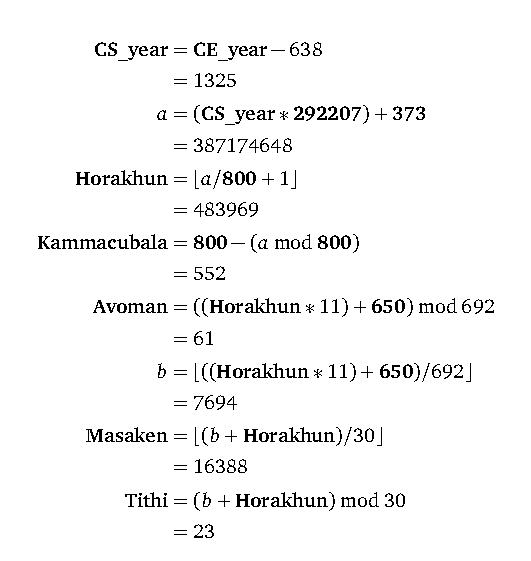
\includegraphics[width=50mm]{formula-sample.pdf}
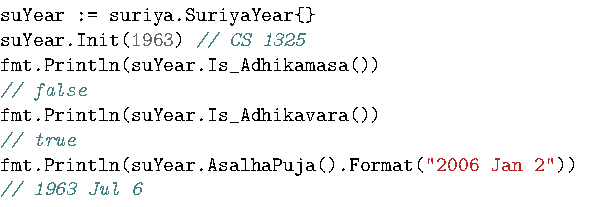
\includegraphics[width=50mm]{code-sample.pdf}
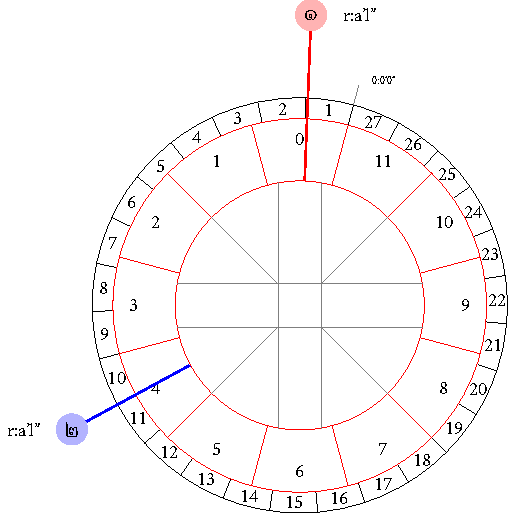
\includegraphics[width=50mm]{duangchata-sample.pdf}

\end{minipage}%
}}%

\clearpage

\chapter{Mahānikāya Uposatha Calendar Tutorial}
\label{sec-1}

This section is a step-by-step guide on how to calculate the uposathas for a
given year.

\section{Collecting information about the year}
\label{sec-1-1}

We need to know the following:

\begin{itemize}
\item the last uposatha of the previous lunar year
\item whether there is an extra lunar month (adhikamāsa),
\item or an extra day (adhikavāra),
\item or neither, and so it is a common year.
\end{itemize}

Find the Full Moon in last year November, this is the last uposatha of the
previous lunar year.

In Thai practice a lunar year can't have both an adhikamāsa and an adhikavāra.

Check Table \ref{tbl-cycle-adhikamasa-adhikavara-short} whether the given year
will have an adhikamāsa or adhikavāra. For more data, see Table
\ref{tbl-cycle-adhikamasa-adhikavara}.

\begin{margintable}[-80mm]
\begin{center}
\begin{tabular}{rrr}
Year & $\Delta$ M & $\Delta$ V\\
\hline
2000 &  & 6\\
2001 &  & \\
2002 & 3 & \\
2003 &  & \\
2004 & 2 & \\
2005 &  & 5\\
2006 &  & \\
2007 & 3 & \\
2008 &  & \\
2009 &  & 4\\
2010 & 3 & \\
2011 &  & \\
2012 & 2 & \\
2013 &  & \\
2014 &  & \\
2015 & 3 & \\
2016 &  & 7\\
2017 &  & \\
2018 & 3 & \\
2019 &  & \\
2020 &  & 4\\
2021 & 3 & \\
2022 &  & \\
2023 & 2 & \\
2024 &  & \\
2025 &  & 5\\
2026 & 3 & \\
2027 &  & \\
2028 &  & \\
2029 & 3 & \\
2030 &  & 5\\
\end{tabular}
\end{center}
\caption{\label{tbl-cycle-adhikamasa-adhikavara-short} 2000-2030.}\legend{\Delta M, \Delta V: years since the last adhikamāsa (M) or adhikavāra (V).}
\end{margintable}

Keep in mind that the data on future adhikavāra years is provisional. Even when
a year would be due for an adhikavāra, the calendar authorities may choose to
add it in a different year.

Now we know that the year is either:

\begin{itemize}
\item a common year,
\item an adhikamāsa year, or
\item an adhikavāra year.
\end{itemize}

Gregorian leap years don't affect the lunar calendar, but it may be useful to
check when planning ahead. Table \ref{tbl-cycle-leap-years} shows a few leap
years.

\section{Common year}
\label{sec-1-2}
\label{common-year}
\subsection{Alternate 30 and 29 day months}
\label{sec-1-2-1}

Counting from the last Full Moon of the previous lunar year (which will be in
November), the first month is 30 days, the second is 29 days:

\begin{center}
\begin{tabular}{lll}
15 days & \mN{} New Moon & First uposatha of the Cold Season\\
15 days & \mF{} Full Moon & End of first month, 30 days\\
14 days & \mN{} New Moon & \\
15 days & \mF{} Full Moon & End of second month, 29 days\\
\end{tabular}
\end{center}

A Full Moon is always on the 15th day. Every second New Moon is on the 14th day.

The \GaWaxingmoon{} Waxing- and \GaWaningmoon{} Waning Moons are on the 8th day.

\begin{fullwidth}
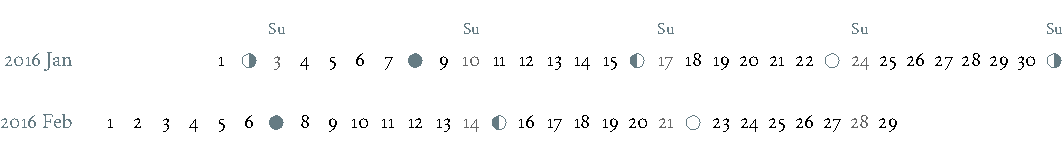
\includegraphics[width=\linewidth]{two-months.pdf}
\end{fullwidth}

Keep alternating 30 and 29 day months. One season is four months, one year is
three seasons: Cold-, Hot- and Rainy Season. See Figure \ref{fig-common-year} or
Table \ref{tbl-month-names} for the Pāli names of months and seasons.

\begin{marginfigure}[-5mm]
\caption{\label{fig-common-year} Common Year.}
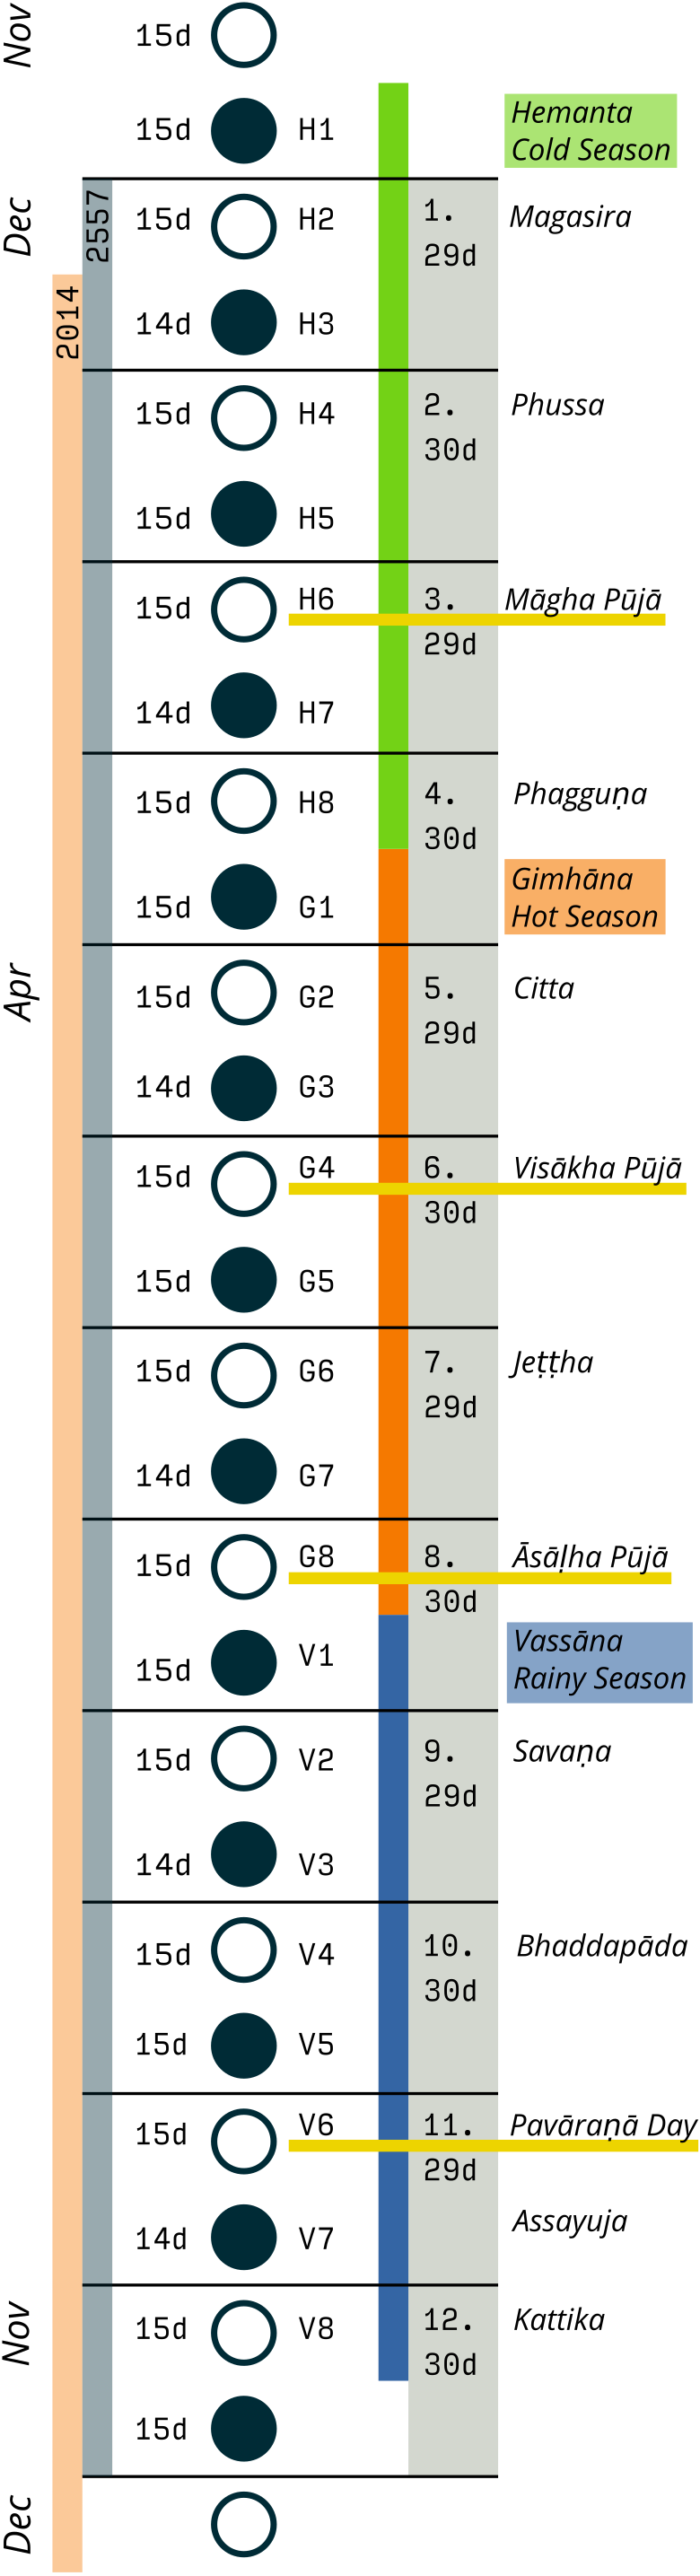
\includegraphics[width=\linewidth]{common-year.png}
\end{marginfigure}

\subsection{Marking the Vassa and Major Moondays}
\label{sec-1-2-2}
\label{marking-the-moondays-common-year}

Mark the months and seasons according to Figure \ref{fig-common-year}.

The key annual events are on the Full Moon of the given lunar months:

\begin{table}[h]
\caption{\label{tbl-major-events} Major Events in a Common Year}
\centering
\begin{tabular}{ll}
Event & Time\\
\hline
Māgha Pūjā & 3rd Full Moon\\
Visākha Pūjā & 6th Full Moon\\
Āsāḷha Pūjā & 8th Full Moon\\
First Day of Vassa & the day after Āsāḷha\\
Pavāraṇā Day & 11th Full Moon\\
Last Day of Vassa & Pavāraṇā Day\\
\end{tabular}
\end{table}

Mark the Vassa (Rainy Season Retreat):

\begin{itemize}
\item The first day of the Vassa is the day after Āsāḷha Pūjā
\item The last day of the Vassa is Pavāraṇā Day
\end{itemize}

The Vassa Retreat therefore is 6 uposathas long (5 + Pavāraṇā), and the Vassāna
season is 8 uposathas.

In a common year, the calendar is finished. 

Note that in \emph{monastic} lunar months, the Full Moon is on the last day of the month.

In \emph{Thai} lunar months, the Full Moon is in the middle of the month, and the New
Moon is on the last day.

\section{Adhikamāsa year}
\label{sec-1-3}
\subsection{Marking the Vassa and Major Moondays}
\label{sec-1-3-1}
\label{marking-the-moondays-adhikamasa-year}

Adding the extra month has three consequences:

\begin{itemize}
\item the Major Moondays shift to the next Full Moon
\item Gimhāna (Hot Season) has 10 uposathas instead of 8
\item the Vassa starts 30 days later
\end{itemize}

\clearpage

\begin{marginfigure}[-22mm]
\caption{\label{fig-adhikamasa-year} Adhikamāsa Year.}
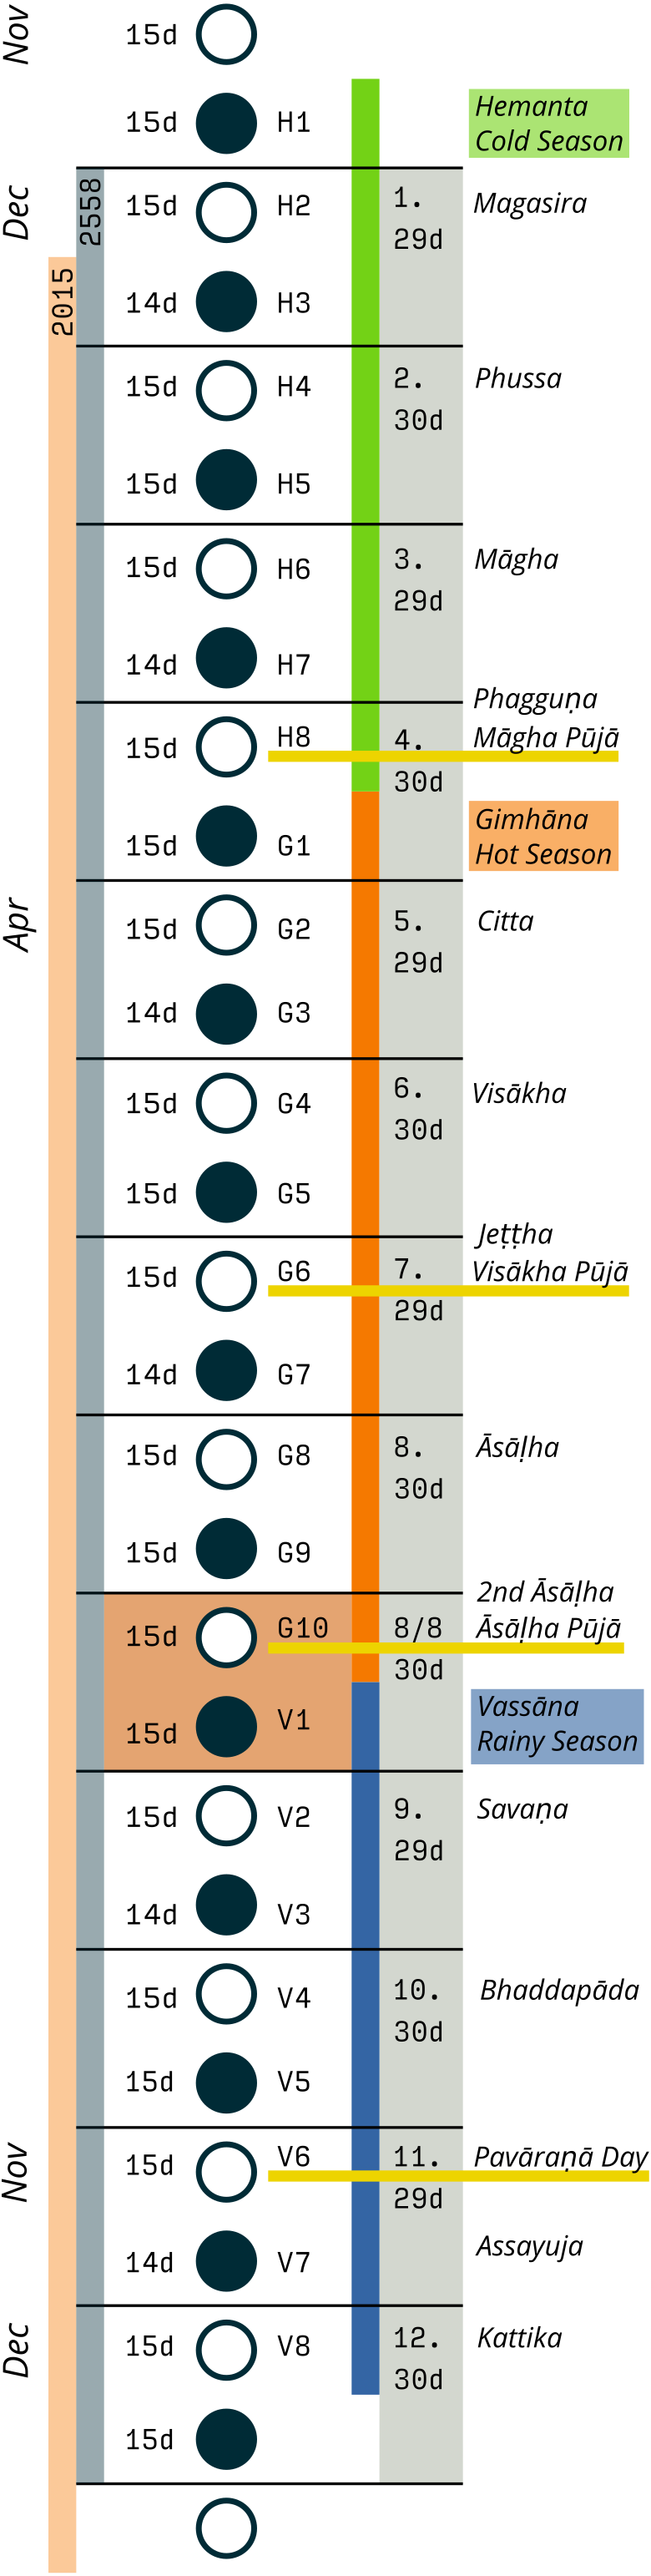
\includegraphics[width=\linewidth]{adhikamasa-year.png}
\end{marginfigure}

The extra month is a 30 day month. In Thai practice, it is appended to the end
of the Hot Season, after the 8th month (Āsāḷha). The convention is to call this
the `second 8th' or `second Āsāḷha', marked as 8/8.

Āsāḷha Pūjā will be held in the 8/8 2nd Āsāḷha month, the first day of the
Vassa being on the following day. The Vassa remains the same length, 8 uposathas.

Āsāḷha Pūjā and Pavāraṇā Day therefore shifted because we added an extra month
to the end of the Hot Season.

From a practical perspective, Māgha Pūjā and Visākha Pūjā are simply moved to
the next month, and are marked in the 4th and 7th month instead of the 3rd and
6th. This is as though the Major Moons had a parallel, separate system of
numbering, in which the adhikamāsa was assumed to be added at the beginning of
the year, but this doesn't influence the actual numbering or length of the
months.

This has the advantage that there will not be a large gap between Visākha and
Āsāḷha Pūjā (now in the 2nd Āsāḷha).

Figure \ref{fig-adhikamasa-year} shows how the sequence of the uposathas and the
major moondays fall in an adhikamāsa year.

\section{Adhikavāra year}
\label{sec-1-4}

\begin{marginfigure}
\caption{\label{fig-adhikavara-year} Adhikavāra Year.}
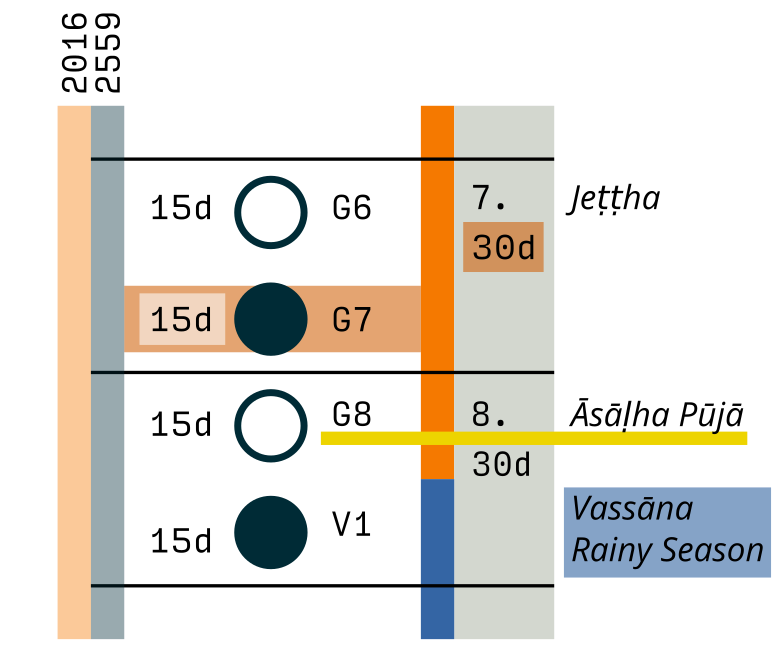
\includegraphics[width=\linewidth]{adhikavara-year.png}
\end{marginfigure}

The extra day is inserted in the 8th month (Āsāḷha), at the New Moon uposatha
before Āsāḷha Full Moon, making the 7th uposatha of the Hot Season a 15-day
uposatha instead of the expected 14-day, and making Āsāḷha a 30-day month that
year.\autocite{hasapannyo-zodiac}

In adhikavāra years the Vassa starts one day later.

\begin{center}
\begin{tabular}{rlr}
order & name & days\\
\hline
6 & Visākha & 29\\
7 & Jeṭṭha & 30\\
8 & Āsāḷha & \textbf{30}\\
9 & Savaṇa & 30\\
10 & Bhaddapāda & 29\\
\end{tabular}
\end{center}

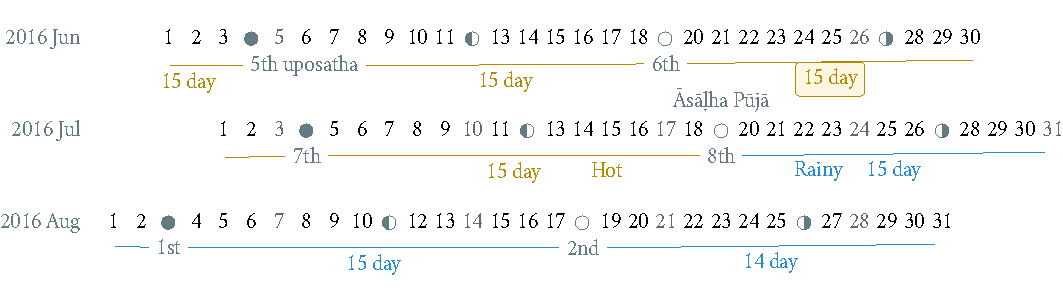
\includegraphics[width=\linewidth]{adding-the-extra-day.pdf}

\clearpage

\chapter{The Mahānikāya Uposatha Calendar Method}
\label{sec-2}
\section{Adding the extra month}
\label{sec-2-1}

The extra month (adhikamāsa) is added 7 times in a 19 year period. This is
determined by the formulas at sec. \ref{suriyayatra-formulas}, which generate a pattern
such that an adhikamāsa year is due in every 2 or 3 years.

It is not sufficient to rely on a shorthand pattern to determine the variation
of 2 or 3 years -- the pattern of 3-3-2 - 3-3-3-2 has been mentioned by Ajahn
Khemanando\autocite{khemanando-adhikamasa}, but this doesn't always match the cycles
produced by the formulas.

Table \ref{tbl-cycle-adhikamasa-adhikavara} shows adhikamāsa years for 1975-2030.

In Thai practice, the extra month is a 30 day month inserted after the
8th month (\emph{Āsāḷha}), at the end of the Hot Season. The convention is
to call this the `second 8th' or `second \emph{Āsāḷha}', marked as 8/8.

\marginpar{%
\begin{center}
\begin{tabular}{rlr}
order & name & days\\
\hline
8 & Āsāḷha & 29\\
8/8 & 2nd Āsāḷha & 30\\
9 & Savaṇa & 30\\
\end{tabular}
\end{center}
}

In adhikamāsa years the Vassa starts 30 days later, after the 2nd
Āsāḷha, on the day after the Full Moon uposatha of 8/8.

\section{Adding the extra day}
\label{sec-2-2}
\label{adding-extra-day}

The extra day (adhikavāra) is added 11 times in every 57 year.

Whether a year should have an extra day is determined by the conditions at
sec. \ref{adhikavara-years}.

In Thai practice a year with an extra month is not allowed to also
have an extra day. If the year should have an extra day, but it
already has an extra month, the extra day is assigned to one of the
flanking years (next or previous, in the case of planning several
years in advance).

In adhikavāra years the Vassa starts one day later.

The extra day is inserted in the 8th month (Āsāḷha), at the New Moon uposatha
before Āsāḷha Full Moon (the 7th uposatha of the Hot Season), making it a 15-day
uposatha instead of the expected 14-day, and making Āsāḷha a 30-day month that
year.\autocite{hasapannyo-zodiac}

The announcement of the adhikavāra years by the calendar authorities is not
entirely predictable. In some of cases the calendar committees add the
adhikavāra in a different year than the regular pattern. However, the years
since 1997 have all been regular.

See Table \ref{tbl-adhikavara-irregularities} for examples of irregular years in the past.

Nonetheless it would be observed that:

\begin{itemize}
\item the count for 11 times in 57 years is maintained to keep the
calendar at pace
\item the extra day will not be in years that also have an extra month.
\end{itemize}

\section{Marking the Vassa and Major Moondays}
\label{sec-2-3}

Common year: sec. \ref{marking-the-moondays-common-year}

Adhikamāsa year: sec. \ref{marking-the-moondays-adhikamasa-year}

Adhikavāra year: the logic is the same as in common years.

\begin{table}[h]
\begin{fullwidth}
\caption{\label{tbl-cycle-adhikamasa-adhikavara} Adhikamāsa and adhikavāra years}

\legend{\Delta M, \Delta V: years since the last
adhikamāsa (M) or adhikavāra (V). nM, nV: n-th place in the adhikamāsa
19-year cycle (M) or the adhikavāra 57 year cycle. 'x' marks years which would
qualify for adhikavāra, but there is already an adhikamāsa, and so the
adhikavāra is carried on to the following year.}

\begin{multicols}{2}

\begin{center}
\begin{tabular}{rrrrrr}
CE year & BE year & nM & $\Delta$ M & nV & $\Delta$ V\\
\hline
1975 & 2518 & 11 & 3 & 49 & \\
1976 & 2519 & 12 &  & 50 & \\
1977 & 2520 & 13 & 2 & 51 & \\
1978 & 2521 & 14 &  & 52 & 5\\
1979 & 2522 & 15 &  & 53 & \\
1980 & 2523 & 16 & 3 & 54 & \\
1981 & 2524 & 17 &  & 55 & \\
1982 & 2525 & 18 &  & 56 & \\
1983 & 2526 & 19 & 3 & 57 & \\
1984 & 2527 & 1 &  & 1 & 6\\
1985 & 2528 & 2 & 2 & 2 & \\
1986 & 2529 & 3 &  & 3 & \\
1987 & 2530 & 4 &  & 4 & \\
1988 & 2531 & 5 & 3 & 5 & \\
1989 & 2532 & 6 &  & 6 & 5\\
1990 & 2533 & 7 &  & 7 & \\
1991 & 2534 & 8 & 3 & 8 & \\
1992 & 2535 & 9 &  & 9 & \\
1993 & 2536 & 10 & 2 & 10 & \\
1994 & 2537 & 11 &  & 11 & 5\\
1995 & 2538 & 12 &  & 12 & \\
1996 & 2539 & 13 & 3 & 13 & \\
1997 & 2540 & 14 &  & 14 & \\
1998 & 2541 & 15 &  & 15 & \\
1999 & 2542 & 16 & 3 & 16 & x\\
2000 & 2543 & 17 &  & 17 & 6\\
2001 & 2544 & 18 &  & 18 & \\
2002 & 2545 & 19 & 3 & 19 & \\
\end{tabular}
\end{center}

\columnbreak

\begin{center}
\begin{tabular}{rrrrrr}
CE year & BE year & nM & $\Delta$ M & nV & $\Delta$ V\\
\hline
2003 & 2546 & 1 &  & 20 & \\
2004 & 2547 & 2 & 2 & 21 & x\\
2005 & 2548 & 3 &  & 22 & 5\\
2006 & 2549 & 4 &  & 23 & \\
2007 & 2550 & 5 & 3 & 24 & \\
2008 & 2551 & 6 &  & 25 & \\
2009 & 2552 & 7 &  & 26 & 4\\
2010 & 2553 & 8 & 3 & 27 & \\
2011 & 2554 & 9 &  & 28 & \\
2012 & 2555 & 10 & 2 & 29 & \\
2013 & 2556 & 11 &  & 30 & \\
2014 & 2557 & 12 &  & 31 & \\
2015 & 2558 & 13 & 3 & 32 & x\\
2016 & 2559 & 14 &  & 33 & 7\\
2017 & 2560 & 15 &  & 34 & \\
2018 & 2561 & 16 & 3 & 35 & \\
2019 & 2562 & 17 &  & 36 & \\
2020 & 2563 & 18 &  & 37 & 4\\
2021 & 2564 & 19 & 3 & 38 & \\
2022 & 2565 & 1 &  & 39 & \\
2023 & 2566 & 2 & 2 & 40 & \\
2024 & 2567 & 3 &  & 41 & \\
2025 & 2568 & 4 &  & 42 & 5\\
2026 & 2569 & 5 & 3 & 43 & \\
2027 & 2570 & 6 &  & 44 & \\
2028 & 2571 & 7 &  & 45 & \\
2029 & 2572 & 8 & 3 & 46 & \\
2030 & 2573 & 9 &  & 47 & 5\\
\end{tabular}
\end{center}

\end{multicols}
\end{fullwidth}
\end{table}

\begin{landscape}
\begin{table}[p]
\caption{\label{tbl-adhikavara-irregularities} Irregular Adhikavāra years. Past calendar sources: myhora.com, thaiorc.com.}
\begin{center}
\begin{tabular}{rrrrrrrrrrrll}
CE year & BE year & K & A & T & nM & $\Delta$ M & nV & $\Delta$ V & Āsāḷha by Calc. & Āsāḷha in Calendar & test & comments\\
\hline
1977 & 2520 & 54 & 252 & 27 & 13 & 2 & 51 &  & 1977-07-30 & 1977-07-30 &  & \\
1978 & 2521 & 647 & 126 & 9 & 14 &  & 52 & 5 & 1978-07-20 & 1978-07-19 & X & adhikavāra is missing from the calendar\\
1979 & 2522 & 440 & 681 & 19 & 15 &  & 53 &  & 1979-07-09 & 1979-07-09 &  & \\
… &  &  &  &  &  &  &  &  &  &  &  & \\
1983 & 2526 & 412 & 144 & 4 & 19 & 3 & 57 &  & 1983-07-24 & 1983-07-24 &  & \\
1984 & 2527 & 205 & 7 & 15 & 1 &  & 1 & 6 & 1984-07-13 & 1984-07-12 & X & adhikavāra is missing\\
1985 & 2528 & 798 & 573 & 26 & 2 & 2 & 2 &  & 1985-08-01 & 1985-07-31 & X & off by -1 day\\
1986 & 2529 & 591 & 436 & 7 & 3 &  & 3 &  & 1986-07-21 & 1986-07-20 & X & off by -1 day\\
1987 & 2530 & 384 & 299 & 18 & 4 &  & 4 &  & 1987-07-10 & 1987-07-10 &  & \\
… &  &  &  &  &  &  &  &  &  &  &  & \\
1993 & 2536 & 742 & 191 & 25 & 10 & 2 & 10 &  & 1993-08-02 & 1993-08-02 &  & \\
1994 & 2537 & 535 & 54 & 6 & 11 &  & 11 & 5 & 1994-07-23 & 1994-07-22 & X & adhikavāra is missing\\
1995 & 2538 & 328 & 609 & 16 & 12 &  & 12 &  & 1995-07-12 & 1995-07-11 & X & off by -1 day\\
1996 & 2539 & 121 & 472 & 27 & 13 & 3 & 13 &  & 1996-07-30 & 1996-07-29 & X & off by -1 day\\
1997 & 2540 & 714 & 346 & 9 & 14 &  & 14 &  & 1997-07-19 & 1997-07-19 &  & \\
\end{tabular}
\end{center}
\end{table}
\end{landscape}


\clearpage

\chapter{The Thai luni-solar calendar}
\label{sec-3}

Luni-solar calendars are constructed so as to count \textbf{years} according to the
\emph{solar} cycle, but to count \textbf{months} according to the \emph{lunar} cycle.

\begin{center}
\begin{tabular}{ll}
tropical year\footnotemark\space of the Earth & 365.24219 days\\
synodic month\footnotemark\space of the Moon & \textasciitilde{}29.53 days, can vary up to 7 hours\\
\end{tabular}
\end{center}\footnotetext[1]{tropical year: the time it takes the Earth to
complete an orbit around the Sun}\footnotetext[2]{synodic month: the time it takes the Moon to reach
the same visual phase}

The epoch of the Thai lunar calendar is 25 March 638 BCE, this is the beginning
of the \emph{Chulasakkarat Era}.\autocite{eade1995calendrical}

The epoch of the \emph{Buddhist Era} is the date when the Buddha attained
Parinibbāna. According to Thai tradition it is 11 March 545 BCE, but the
difference between CE and BE in Thailand is now fixed at 543
years.\autocite{eade1995calendrical}

Thus the conversion between the eras:

\begin{center}
\begin{tabular}{lll}
CE 1963 & Common Era & \\
BE 2506 & Buddhist Era & CE + 543\\
CS 1325 & Chulasakkarat Era & CE - 638\\
\end{tabular}
\end{center}

The Thai luni-solar calendar is \emph{procedural}. It uses a few constant,
key numbers derived from astronomical observations, and applies a
series of mechanical calculations (i.e. the ``rules'') again and again
to generate the dates of lunar phases and new years.

\begin{quote}
This working is deliberately concise, since it thereby reflects how
the calculation would have been made by a South East Asian calendrist.
Each stage is subjected to an operation learnt by rote, and the
underlying theory disappears from view. The rote operations, however,
will provide a valid answer for any date in any year. It seemed
greatly preferable to set out the procedure thus starkly, rather than
to give a detailed exposition of what is involved.\autocite{eade-interpolation}
\end{quote}

Southeast Asian astronomers refined a fraction to obtain the length of the year.
Taking 800 years as one Era, and 292207 days in the Era, they expressesed the
length of one year in days as\autocite{eade-interpolation}:

\begin{equation}
\frac{292207}{800} = 365.25875\ \text{days}
\end{equation}

This is 0.01656 days longer than the modern measurement (accumulating
1 day in \textasciitilde{}60 years). Remarkably, the \emph{suriyayatra} accounts for this
and generates accurate results:

\begin{quote}
For instance, a Pagan inscription of 14 April 1288 AD maintains that
at midnight the Sun's position was 0 signs, 19 degrees and 59 minutes:
the computer program returns
0~19~59.\autocite[p. 2]{eade1995calendrical}
\end{quote}

Let's see if we can get the same results. 14 April 1288 was 41 days into the
lunar year, counting from Citta 1. While checking that, we might as well see day
103, i.e. 15 June 1288, which should turn out to be Āsāḷha Pūjā.

\begin{marginfigure}
\caption{1288 April 14}

\resizebox{\linewidth}{!}{\DuangChata[Sun={0/19/58}, Moon={5/11/27}, simple, show angles]}

\footnotesize
\bigskip

\begin{tabular}{l l}
Sun: & 0:19\degree 58\minute\\
Moon: & 5:11\degree 27\minute\\
Tithi: & 12
\end{tabular}

\bigskip

The Moon is in the 13. nakshatra, Hasta.

\end{marginfigure}

\begin{marginfigure}
\caption{1288 June 15}

\resizebox{\linewidth}{!}{\DuangChata[Sun={2/19/9}, Moon={8/19/1}, simple, show angles]}

\footnotesize
\bigskip

\begin{tabular}{l l}
Sun: & 2:19\degree 9\minute\\
Moon: & 8:19\degree 1\minute\\
Tithi: & 15
\end{tabular}

\bigskip

The Moon is in the 20. nakshatra, Pūrva Ashādhā.

\end{marginfigure}

The code example is at \ref{golang-1288}. It prints:

\begin{verbatim}
Year: 1288
Adhikamāsa: false
Adhikavāra: false
---
Year, Day: 1288, 41
True Sun: 0:19°58'
True Moon: 5:11°27'
Tithi: 12
---
Year, Day: 1288, 103
True Sun: 2:19°9'
True Moon: 8:19°1'
Tithi: 15
\end{verbatim}

On day 103, tithi 15 means 15 lunar days since last New Moon, i.e. it is Full
Moon. The Sun and Moon are angularly opposite, which also means Full Moon, and
it appears in the 20. nakshatra, so the month is Āsāḷha.

As a reality check, we can look up the phase at NASA:\footnote{\href{http://astropixels.com/ephemeris/phasescat/phases1201.html}{AstroPixels - Moon Phases: 1201 to 1300}}

{\centering
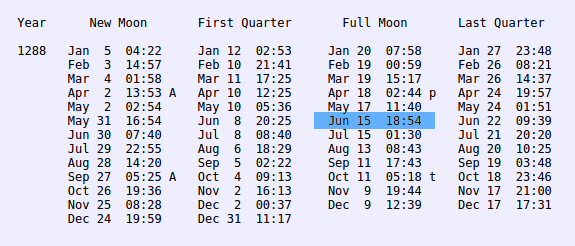
\includegraphics[width=0.8\linewidth]{1288-astropixels.png}
\par}

Nonetheless, the calendar dates published in Thailand (historical or
recent) in a given year reflect not only these principles, but also
adjustments and omissions which cannot be foreseen or retraced.

\begin{quote}
The historical record however, frequently defies prediction, forcing
the conclusion that the pressure upon the \emph{horas} (astronomers /
astrologers) was not to follow the ``rules'' but merely, within some
more leisurely constraints, to ensure that the calendar did not get
out of control.\autocite{eade1995calendrical}
\end{quote}

Eade discusses a calendar error in CS 855 (CE 1493) when the formulas have
determined a \emph{twelfth} adhikavāra year in a 57 year period, which was not
noticed by several astronomers at the time, who were using the ``11 times in 57
years'' rule of thumb for adhikavāra years. This resulted in wrong dates being
used on any inscriptions made until the error was corrected in the
calendar.\autocite{eade2007irregular}

\section{Names of the months}
\label{sec-3-1}

The name of a given month is determined by the astrological sign which
the Full Moon enters at midnight. See Table \ref{tbl-month-names}.

The lunar year starts in April with Citta-māsa, which is 0 degrees (the vernal
equinox) on the wheel of the zodiac (see sec. \ref{duangchata}), corresponding
to Aries.

\begin{table}[h]
\caption{\label{tbl-month-names} Lunar and Solar Months and Zodiacs\autocite{hasapannyo-zodiac}}
\centering
\begin{tabular}{lrrlll}
Season &  &  & Lunar Month & Solar Month & Solar Zodiac\\
 &  & days &  &  & (Western / Sanskrit)\\
\hline
Gimha-utu & 1 & 30 & Citta-māsa & April & Aries / Meṣa\\
Hot Season & 2 & 29 & Visākha-māsa & May & Taurus / Vṛṣabha\\
 & 3 & 30 & Jeṭṭha-māsa & June & Gemini / Mithuna\\
 & 4 & 29 & Āsāḷha-māsa & July & Cancer / Karkaṭa\\
\hline
Vassāna-utu & 5 & 30 & Savaṇa-māsa & August & Leo / Siṃha\\
Rainy Season & 6 & 29 & Bhaddapāda-māsa & September & Virgo / Kanyā\\
 & 7 & 30 & Assayuja-māsa & October & Libra / Tulā\\
 & 8 & 29 & Kattika-māsa & November & Scorpio / Vṛścika\\
\hline
Hemanta-utu & 9 & 30 & Magasira-māsa & December & Sagittarius / Dhanus\\
Cold Season & 10 & 29 & Phussa-māsa & January & Capricorn / Makara\\
 & 11 & 30 & Māgha-māsa & February & Aquarius / Kumbha\\
 & 12 & 29 & Phagguṇa-māsa & March & Pisces / Mīna\\
\end{tabular}
\end{table}

\section{The first and last day of a lunar month}
\label{sec-3-2}
\label{lunar-month-first-last}

In monastic practice, the Full Moon day is on the last day of a given
month. The next month starts on the following day (first day of the
waning phase), thus the first uposatha will be on a New Moon.

In many Thai calendars, the New Moon day is the last day of the month,
and the Full Moon day is in the middle. This only changes the
numbering of the months, not the actual moondays. In these calendars
the thresholds of months are shifted two weeks forward relative to the
monastic calendar.

This can be particularly important to watch at the end of the lunar year:

The New Moon of the 12th \emph{Thai} lunar month is the New Moon (1st uposatha) of
the 1st \emph{monastic} lunar month.

\begin{table}[h]
\caption{\label{monastic-thai-year} Monastic and Thai lunar months in a year}
\centering
\begin{tabular}{rllrr}
Nth & phase & month & Monastic & Thai\\
\hline
1 & New &  & 1 & 12\\
2 & Full & Magasira & 1 & 1\\
3 & New &  & 2 & 1\\
4 & Full & Phussa & 2 & 2\\
5 & New &  & 3 & 2\\
6 & Full & Māgha & 3 & 3\\
7 & New &  & 4 & 3\\
8 & Full & Phagguṇa & 4 & 4\\
\end{tabular}
\end{table}


\begin{table}[p]
\caption{\label{tbl-calendars-1958} Adhikamāsa and adhikavāra in the period 1958 to 1978 (CS 1320-1340).\autocite{eade-interpolation}}\legend{m for adhikamāsa, d for adhikavāra years, \Delta m and \Delta d for years since last adhikamāsa and adhikavāra.}
\centering
\begin{tabular}{rrrrrlrr}
 & $\Delta$ d &  & $\Delta$ m & year & type & Asalha & 2nd Asalha\\
\hline
 &  & 0 &  & 1320 & m & 19:42 & 22:24\\
0 &  & 1 &  & 1321 & d & 21:05 & \\
1 &  & 2 &  & 1322 &  & 20:40 & \\
2 &  & 3 & 3 & 1323 & m & 19:12 & 22:00\\
3 &  & 4 &  & 1324 &  & 20:38 & \\
4 & 4 & 5 &  & 1325 & d & 19:34 & \\
5 &  & 6 & 3 & 1326 & m & 19:38 & 22:05\\
6 &  & 7 &  & 1327 &  & 21:15 & \\
7 &  & 8 & 2 & 1328 & m & 19:20 & 22:55\\
8 &  & 9 &  & 1329 &  & 21:48 & \\
9 & 5 & 10 &  & 1330 & d & 20:26 & \\
10 &  & 11 & 3 & 1331 & m & 19:59 & 22:50\\
11 &  & 12 &  & 1332 &  & 21:20 & \\
12 &  & 13 &  & 1333 &  & 20:02 & \\
13 &  & 14 & 3 & 1334 & m & 19:03 & 21:33\\
14 & 5 & 15 &  & 1335 & d & 20:40 & \\
15 &  & 16 &  & 1336 &  & 20:44 & \\
16 &  & 17 & 3 & 1337 & m & 19:44 & 22:19\\
17 &  & 18 &  & 1338 &  & 21:11 & \\
18 &  & 19 & 2 & 1339 & m & 19:45 & 22:35\\
19 & 5 &  &  & 1340 & d & 21:05 & \\
\end{tabular}
\end{table}


\clearpage

\chapter{Suriyayatra formulas}
\label{sec-4}
\label{suriyayatra-formulas}
\section{Overview}
\label{sec-4-1}

The formulas take two inputs: the year, and the n$^{\text{th}}$ day in the lunar year.
They go through a series of operations step by step to produce certain values
which describe properties of the lunar year and the given day.

For $\mathbf{day} = 0$, the results are used to determine whether the year is
common, adhikamāsa or adhikavāra. They can also give us the angular position of
the Sun and the Moon on the given day.

\begin{marginfigure}
\raggedright
\caption{\label{fig-wheel-2014-asalha} 2014 July 11, Āsāḷha Full Moon}

\resizebox{\linewidth}{!}{\DuangChata[Sun={2/25/22}, Moon={8/16/6}, simple, show angles]}

\footnotesize
\bigskip

\begin{tabular}{l l}
True Sun: & 2:25\degree 22\minute\\
True Moon: & 8:16\degree 6\minute\\
Raek: & 20:12\minute\\
Masaken: & 17022\\
Avoman: & 391\\
Horakhun: & 502683\\
Kammacubala: & 69195\\
Uccabala: & 1102\\
Tithi: & 14
\end{tabular}

\bigskip

At midnight the Moon would be seen in the 20. Nakshatra, Pūrva Ashādhā, around the stars δ and ε Sagittarii.

\end{marginfigure}


For example in a common year, when we calculate the Moon's position for
$\mathbf{day} = 103$, it should tell us that it is Full Moon, and it is found in
the region of the sky associated with Āsāḷha month.

Significant values are assigned names.\autocite{eade1989ephemeris} The following
three will determine the adhikamāsa and adhikavāra:

\savenotes

\begin{description}
\item[{Kammacubala \thai{กัมมัชพล}}] Remaining 800ths of a day
\item[{Avoman \thai{อวมาน}}] For the Moon's mean motion
\item[{Tithi\footnote{a.k.a. Thaloengsok or New Year's Day} \thai{ดีถี}}] Age of the Moon, at the start of the year if $\mathbf{day} = 0$
\end{description}

As we follow the steps, we will also obtain:

\begin{description}
\item[{Horakhun \thai{อหรคุณ}}] Elapsed days of the era
\item[{Uccabala \thai{อุจจพล}}] Age of the Moon's Apogee
\item[{Masaken \thai{มาสเกณฑ์}}] Elapsed months of the era

\item[{MeanSun, TrueSun, MeanMoon, TrueMoon}] Mean and True angular position of the Sun and the Moon
\item[{Raek}] The position of the Moon in terms of the 27 lunar mansions, which will determine the month
\end{description}

\spewnotes

The zodiac wheel (a.k.a \emph{duang chata}, sec. \ref{duangchata}) is divided into 12
segments called \emph{rasi} (\thai{ราศี}), each marking 30 degrees.

The wheel is also divided into 27 lunar mansions called \emph{nakshatra}
(\thai{นักษัตร}).

Angular positions are given in a notation that expresses the rasi number plus
the degrees and arcminutes. These values are also called the \emph{rasi}, \emph{angsa} and
\emph{lipda}.

The notation $r:a\degree l\minute = r*30 + a + l/60$, thus $85\degree 22\minute$ is
$2:25\degree 22\minute$.


Only basic operations in a series of simple steps are necessary to produce these
results. It can be carried out entirely on paper, although the aim here is to
get the machine to do it for us eventually.

This is a simplistic clockwork model of the solar system. It is not a framework
to model orbital mechanics, and doesn't account for such things as the varying
speed of the Moon in its elliptical orbit.

Therefore there can be inaccuracies for a given day between its results and
observations made with telescopes (or indeed by plain sight) about what is
actually going on ``out there'', but nonetheless it keeps the long-term calendar
in sync with the periodic cycles of the celestial bodies.

Consider the ancient \emph{hora} \thai{โหรา} (astronomer / astrologer) in a rural village who is
practising these steps. He doesn't have the equipment to make precise
astronomical observations. He is not educated in the underlying theory of the
complex interaction of the Sun, Earth and the Moon. He is only trained in
following the steps, and still this allows him to obtain the necessary
information to describe the progression of these events in any year.

\section{Calculating the properties of the year}
\label{sec-4-2}

First we will see if we should add and extra month or extra day to keep the
lunar year in sync with the solar year.

Then we will calculate the position of the Moon on that day, and see if we are
in Āsāḷha month, and not at some other Full Moon.

We can confirm this by looking up the Moon phases published by NASA and check if
the Āsāḷha Pūjā date had in fact been a Full Moon.

Let's take the year CE 1963 (CS 1325) as an example and calculate its
properties. We should find that it is an adhikavāra year. If you calculate the
following year CE 1964 (CS 1326) as an excercise, you should find that it is
adhikamāsa.

Notation recap:

$a \bmod b$ produces the \emph{remainder part} of $a/b$.\\
E.g. $14 \bmod 5 = 4$, because $14/5 = 2*5 + 4$.

$\lfloor a \rfloor$ \emph{floors} (or truncates) a fraction value, meaning we discard
the fraction part and only keep the integer part.\\
E.g. $\lfloor 12.8 \rfloor = 12$.

$|a|$ is the \emph{absolute} value of $a$.\\
E.g. $|-4.21| = 4.21$ and $|4.21| = |4.21|$.


Era Constants. For readability, in the formulas we will use their values directly, set in \textbf{bold}.

\begin{align*}
  \mathbf{EraYears} & = 800 & \mathbf{EraDays} & = 292207 & \mathbf{MonthLength} & = 30
\end{align*}

Constant offsets, which have to be added because their value was not 0 at the beginning of the Era:

\begin{align*}
  \mathbf{EraHorakhun} & = 373 & \mathbf{EraUccabala} & = 2611 & \mathbf{EraAvoman} & = 650 
\end{align*}

3232 is a "base" for 360 degrees.\autocite[p. 48]{eade1995calendrical}

The relationship between periods of \textbf{solar days} and \textbf{tithi}:
"For every 692 solar days that elapse there are also 703 tithi.
Since 703 / 692 can be expressed as 692 + 11 / 692, the ratio is simplified to these terms ...
11 is the daily increase (excess tithi over days)."\autocite[p. 48]{eade1995calendrical}

\begin{equation}
\frac{703}{692} = \frac{692 + 11}{692}
\end{equation}

Let's begin then:

\begin{align}
\begin{split}
   \mathbf{CS\_year} &= \mathbf{CE\_year} - 638\\
                     &= 1325
\end{split}\\
\begin{split}
                   a &= (\mathbf{CS\_year} * \mathbf{292207}) + \mathbf{373}\\
                     &= 387174648
\end{split}\\
\begin{split}
\mathbf{Horakhun}    &= \lfloor a / \mathbf{800} + 1 \rfloor\\
                     &= 483969
\end{split}\\
\begin{split}
\mathbf{Kammacubala} &= \mathbf{800} - (a \bmod \mathbf{800})\\
                     &= 552
\end{split}\\
\begin{split}
\mathbf{Uccabala}    &= (\mathbf{Horakhun} + \mathbf{2611}) \bmod 3232\\
                     &= 1780
\end{split}\\
\begin{split}
                   a &= (\mathbf{Horakhun} * 11) + \mathbf{650}\\
                     &= 5324309
\end{split}\\
\begin{split}
\mathbf{Avoman}      &= a \bmod 692\\
                     &= 61
\end{split}\\
\begin{split}
                   b &= \lfloor a / 692 \rfloor\\
                     &= 7694
\end{split}\\
\begin{split}
\mathbf{Masaken}     &= \lfloor (b + \mathbf{Horakhun}) / \mathbf{30} \rfloor\\
                     &= 16388
\end{split}\\
\begin{split}
\mathbf{Tithi}       &= (b + \mathbf{Horakhun}) \bmod \mathbf{30}\\
                     &= 23
\end{split}
\end{align}

Now we can determine if the year qualifies for adhikamāsa or adhikavāra.

\section{Adhikamāsa conditions}
\label{sec-4-3}
\label{adhikamasa-years}

(Thai: atikamat \thai{อธิกมาส})

The year could be adhikamāsa:

\begin{itemize}
\item \logic{IF} the \textbf{Tithi} is between 24 and 29 inclusive,
\item \logic{OR} between 0 and 5 inclusive,
\item \logic{then} it could be adhikamāsa.
\end{itemize}

However:

\begin{itemize}
\item \logic{IF} the next year also satisfies the above,
\item \logic{then} this year will not be adhikamāsa, and the next year will be.
\end{itemize}

Adhikamāsa years are not allowed to be contiguous, and max. 2 years are allowed
between them. If next year also qualifies for adhikamāsa, then it will be
assigned there and not to the current year.

In the above example for year CS 1325, the \textbf{Tithi} is 23, which doesn't satisfy
the first condition, and so it can't be adhikamāsa.

\section{Adhikavāra conditions}
\label{sec-4-4}
\label{adhikavara-years}

(Thai: atikawan \thai{อธิกวาร})

Determine if it is a leap year:

\begin{itemize}
\item \logic{IF} the \textbf{Kammacubala} is less than or equal to 207,
\item \logic{THEN} it is a leap year.
\end{itemize}

The year could be adhikavāra:

\begin{itemize}
\item \logic{IF} it is a leap year \logic{AND} the \textbf{Avoman} is less than or equal to 126,
\item \logic{then} it could be adhikavāra.
\item \logic{ELSE IF} it is \logic{NOT} a leap year \logic{AND} the \textbf{Avoman} is less than 137,
\item \logic{then} it could be adhikavāra.
\end{itemize}

\marginpar{\footnotesize
``Carried adhikavāra'' meaning that last year qualified both for adhikamāsa and
adhikavāra, so it was not allowed to be assigned the adhikavāra, which was
``carried on'' and will now be assigned to this year.

In Thailand, years with an extra month are not allowed to also have an extra
day, and the adhikavāra may be assigned to one of the flanking years. So in
theory it could be assigned to the following or preceding year, but the general
practice is to ``carry on'' the adhikavāra and assign it to the following year.
}

However:

\begin{itemize}
\item \logic{IF} the year is adhikamāsa,
\item \logic{then} it can't be adhikavāra.
\item \logic{ELSE IF} there is a carried adhikavāra from last year,
\item \logic{then} this year will be adhikavāra.
\end{itemize}

In the above example for year CS 1325: The year is not adhikamāsa, so we can
examine it further. The \textbf{Kammacubala} is 552 so it is not a leap year. The
\textbf{Avoman} is 61, so the year qualifies to be assigned an adhikavāra.

Now we know if the year is adhikamāsa, adhikamāsa or common, and we can plan the
\emph{uposathas} as shown in the diagram on
p.\pageref{dia-common-adhikamasa-adhikavara}.

Checking the past calendars for year CS 1325 (see Table
\ref{tbl-calendars-1958}), we see that indeed it was adhikavāra, conforming to
the formulas.

Nonetheless, the future remains uncertain and the past inscrutable at times.
When the calendar comittees plan several years ahead, they may assign the
adhikavāra to a different year for reasons that remain obscured, causing at
least two irregular years. This can be observed in past calendars (Table
\ref{tbl-adhikavara-irregularities}), but recently this hasn't been happening,
and the years follow the prediction of the formulas.

\section{Calculating the Position of the Sun and the Moon}
\label{sec-4-5}

Eade describes the formulas at the end of his paper \emph{Rules for interpolation in
the Thai calendar}\autocite{eade2000rules}, but his notation is a puzzle in itself,
with its implied conversions and obscure progression from one step to the next.

The folks at \href{http://astronomy.stackexchange.com/}{Astronomy Stack Exchange} helped to decipher it:

\begin{itemize}
\item \href{http://astronomy.stackexchange.com/questions/11753/how-to-interpret-this-old-degree-notation}{How to interpret this old degree notation?}
\item \href{http://astronomy.stackexchange.com/questions/12052/from-mean-moon-to-true-moon-in-an-old-procedural-calendar}{From Mean Moon to True Moon in an old procedural calendar}
\end{itemize}

This allows us to continue examining the year CE 1963 (CS 1325).

We know now that the year needed an adhikavāra extra day, so Āsāḷha Pūjā is one
day later, on day 104, which is 1963 July 6. Let's find the position of the Sun
and the Moon on that day, to see if the Moon reached its Full phase, and if it
is in the region of the sky associated with the correct month (i.e. the
nakshatra).

First we establish the properties of the day:

\begin{align}
\begin{split}
   \mathbf{elapsedDays} &= \mathbf{Day} - \mathbf{Year\_Tithi}\\
                        &= x
\end{split}\\
\begin{split}
   \mathbf{Horakhun}    &= \mathbf{Year\_Horakhun} + \mathbf{elapsedDays}\\
                        &= x
\end{split}\\
\begin{split}
  \mathbf{Kammacubala}  &= \mathbf{800} - (\mathbf{CS\_Year} * \mathbf{292207} + \mathbf{373}) \bmod \mathbf{800} + \mathbf{elapsedDays} * \mathbf{800}\\
                        &= x
\end{split}\\
\begin{split}
  \mathbf{Uccabala}     &= (\mathbf{Horakhun} + \mathbf{2611}) \bmod 3232\\
                        &= x
\end{split}\\
\begin{split}
                      a &= (\mathbf{Horakhun} * 11) + 650\\
        \mathbf{Avoman} &= a \bmod 692\\
                        &= x
\end{split}\\
\begin{split}
                      b &= \lfloor a / 692 \rfloor + \mathbf{2611} + \mathbf{Horakhun}\\
       \mathbf{Masaken} &= \lfloor b / \mathbf{30} \rfloor\\
                        &= x
\end{split}\\
\begin{split}
         \mathbf{Tithi} &= b \bmod \mathbf{30}\\
                        &= x
\end{split}
\end{align}

Find the position of the \textbf{Mean} and \textbf{True Sun}:

Degree to radian conversion noted as $a_{rad} = a * \frac{\pi}{180}$.

Note that 60 converts values between degrees and arcminutes: 

\[ a\degree*60=b\minute \quad \text{and} \quad b\minute/60 = a\degree \]

\begin{align}
\begin{split}
                      a &= \mathbf{elapsedDays} * \mathbf{800} + \mathbf{Year\_Kammacubala}\\
       \mathbf{MeanSun} &= (a / \mathbf{292207}) * 360\degree - 3\minute\\
                        &= x
\end{split}\\
\begin{split}
                         a &= | \mathbf{MeanSun} - 80\degree | \\
          \mathbf{TrueSun} &= \mathbf{MeanSun} + \frac{\lfloor 134 * \mathit{sin}(a_{rad}) \rfloor}{60}\\
                           &= x
\end{split}
\end{align}

Find the position of the \textbf{Mean} and \textbf{True Moon}:

\begin{align}
\begin{split}
                  a &= \frac{\mathbf{Avoman} + \lfloor \mathbf{Avoman} / 25 \rfloor}{60}\\
  \mathbf{MeanMoon} &= \mathit{NormalizeDegree}( \mathbf{TrueSun} + a\degree + \mathbf{Tithi} * 12\degree - 40\minute )\\
                    &= x
\end{split}
\end{align}

One \textbf{Tithi} is 12\degree, from $360\degree / 30 = 12\degree$.

The \textbf{meanUccabala} in one step:

\begin{align}
\begin{split}
  \mathbf{meanUccabala} &= \left( \frac{(\mathbf{Year\_Uccabala} + \mathbf{elapsedDays}) * 3}{808} * 30 * 60 + 2 \right) / 60\\
                        &= x
\end{split}
\end{align}

Breaking it down:

\begin{itemize}
\item Multiply by 30 to conform with the notation $r:a\degree l\minute = 30*r + a + l/60$.
\item Division by 808 probably helps to express the length of the lunar month, since $808 / 30 = 26.9333$.
\item Multiply by 60 to convert to arcmin
\item Add 2, possibly correction for geographical position
\item Divide by 60 to convert back to degree
\end{itemize}

\begin{align}
\begin{split}
                 a &= \mathbf{MeanMoon} - \mathbf{meanUccabala}\\
 \mathbf{TrueMoon} &= \mathbf{MeanMoon} - \frac{296 * \mathit{sin}(a_{rad})}{60}\\
                   &= x
\end{split}\\
\begin{split}
     \mathbf{Raek} &= \mathbf{TrueMoon} / 13\degree 20\minute + 1\\
                   &= x
\end{split}
\end{align}

13\degree 20\minute is one nakshatra or lunar mansion, $360\degree / 27$.

\begin{fullwidth}%
% ============================================== %
\begin{minipage}{0.33\linewidth}
Day 103, 1963 July 5\\

\resizebox{\linewidth}{!}{\DuangChata[Sun={0/0/0}, Moon={0/0/0}, simple, show angles]}

\footnotesize
\bigskip

\begin{tabular}{l l}
Sun: & 0:0\degree 0\minute\\
Moon: & 0:0\degree 0\minute\\
Tithi: & 0
\end{tabular}

\bigskip

X. nakshatra, X X.

\end{minipage}%
% ============================================== %
\begin{minipage}{0.33\linewidth}
Day 104, 1963 July 6\\

\resizebox{\linewidth}{!}{\DuangChata[Sun={0/0/0}, Moon={0/0/0}, simple, show angles]}

\footnotesize
\bigskip

\begin{tabular}{l l}
Sun: & 0:0\degree 0\minute\\
Moon: & 0:0\degree 0\minute\\
Tithi: & 0
\end{tabular}

\bigskip

20. nakshatra, Pūrva Ashādhā.

\end{minipage}%
% ============================================== %
\begin{minipage}{0.33\linewidth}
Day 105, 1963 July 7\\

\resizebox{\linewidth}{!}{\DuangChata[Sun={0/0/0}, Moon={0/0/0}, simple, show angles]}

\footnotesize
\bigskip

\begin{tabular}{l l}
Sun: & 0:0\degree 0\minute\\
Moon: & 0:0\degree 0\minute\\
Tithi: & 0
\end{tabular}

\bigskip

X. nakshatra, X X.

\end{minipage}%
% ============================================== %
\end{fullwidth}

Let's look up what NASA has for 1963 July 6:\footnote{\href{http://astropixels.com/ephemeris/phasescat/phases1901.html}{AstroPixels - Moon Phases: 1901 to 2000}}

{\centering
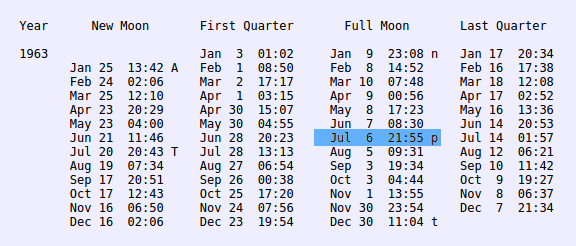
\includegraphics[width=0.8\linewidth]{1963-astropixels.png}
\par}

\clearpage

\chapter{The Duang Chata}
\label{sec-5}
\label{duangchata}

\begin{figure}[h]
\caption{Duang Chata \thai{ดวงชะตา}.}
\resizebox{\linewidth}{!}{\DuangChata[Sun={2/0/0}, Moon={4/5/10}, fancy]}

Horakhun\\
Tithi

\end{figure}

Sun on Thai duang: \thai{๑}\\
Moon on Thai duang: \thai{๒}

Rasi is 0-11, Nakshatra is 1-27. Sun = \theSun, Moon = \theMoon.

0:1\degree 2\minute = Rasi:Angsa\degree Lipda\minute or Rasi:Degree\degree Minute\minute.

\section{Tithi progression}
\label{sec-5-1}

30 Tithi, 15 is Full Moon

Duang at Tithi: 0 3 6 9 12 15 18 21 24 27 29(?)

\section{Rasi}
\label{sec-5-2}

Rasi \thai{ราศี}

\begin{table}[h]
\caption{\label{tbl-rasi-names} Names of the 12 Rasi.}
\centering
\begin{tabular}{rlll}
 & Western & Sanskrit & Thai\\
\hline
0 & Aries & Meṣa & \thai{เมษ}\\
1 & Taurus & Vṛṣabha & \thai{พฤษภ}\\
2 & Gemini & Mithuna & \thai{เมถุน}\\
3 & Cancer & Karkaṭa & \thai{กรกฎ}\\
4 & Leo & Siṃha & \thai{สิงห์}\\
5 & Virgo & Kanyā & \thai{กันย์}\\
6 & Libra & Tulā & \thai{ตุลย์}\\
7 & Scorpio & Vṛścika & \thai{พิจิก}\\
8 & Sagittarius & Dhanus & \thai{ธนู}\\
9 & Capricorn & Makara & \thai{มังกร}\\
10 & Aquarius & Kumbha & \thai{กุมภ์}\\
11 & Pisces & Mīna & \thai{มีน}\\
\end{tabular}
\end{table}

The circle is divided into 12 segments called \emph{rasi}, each marking 30 degrees.
Their numbering starts from 0, to express $x*30\degree$. See Table
\ref{tbl-rasi-names}.

0 degree (Aries) is the vernal equinox.

The notation $x:y\degree z\minute = x*30 + y + z/60$, thus 36\degree 5\minute is
$1:6\degree 5\minute$.

\section{Nakshatra, lunar mansions}
\label{sec-5-3}

Nakshatra \thai{นักษัตร}


The Moon moves about 13\degree$\backslash$ a day, which in general means it traverses one
lunar mansion per day.


\url{https://en.wikipedia.org/wiki/Nakshatra} 

\url{https://th.wikipedia.org/wiki/\%E0\%B8\%94\%E0\%B8\%B2\%E0\%B8\%A7\%E0\%B8\%99\%E0\%B8\%B1\%E0\%B8\%81\%E0\%B8\%82\%E0\%B8\%B1\%E0\%B8\%95\%E0\%B8\%A4\%E0\%B8\%81\%E0\%B8\%A9\%E0\%B9\%8C}

\begin{center}
\begin{tabular}{rll}
 & Sanskrit & Thai\\
\hline
1 & Ashvinī & \thai{อัศวินี}\\
2 & Bharanī & \thai{ภรณี}\\
3 & Kṛttikā & \thai{กฤติกา}\\
4 & Rohinī & \thai{โรหิณี}\\
5 & Mrigashīra & \thai{มฤคศีรษะ}\\
6 & Ārdrā & \thai{อาทรา}\\
7 & Punarvasu & \thai{ปุนวสุ}\\
8 & Pushya & \thai{ปุษยะ}\\
9 & Āshleshā & \thai{อาศเลศา}\\
10 & Maghā & \thai{มฆา}\\
11 & Pūrva Phalgunī & \thai{บูรพผลคุณี}\\
12 & Uttara Phalgunī & \thai{อุตรผลคุณี}\\
13 & Hasta & \thai{หัสตะ}\\
14 & Chitrā & \thai{จิตรา}\\
15 & Svātī & \thai{สวาตี}\\
16 & Vishākhā & \thai{วิศาขา}\\
17 & Anurādhā & \thai{อนุราธา}\\
18 & Jyeshtha & \thai{เชษฐะ}\\
19 & Mūla & \thai{มูละ}\\
20 & Pūrva Ashādhā & \thai{บูรพาษาฒ}\\
21 & Uttara Ashādhā & \thai{อุตราษาฒ}\\
22 & Shravana & \thai{ศรวณะ}\\
23 & Dhanistha & \thai{ศรวิษฐะ}\\
24 & Shatabhisha & \thai{ศตภิษัช}\\
25 & Pūrva Bhādrapadā & \thai{บูรพภัทรบท}\\
26 & Uttara Bhādrapadā & \thai{อุตรภัทรบท}\\
27 & Revatī & \thai{เรวตี}\\
\end{tabular}
\end{center}

\clearpage

\chapter{In Golang}
\label{sec-6}
\label{suriya-go-example}

Going through all this may be intriguing to calculate once, but mention
repeating it every year, then checking and proofing it, and one is reminded of a
phrase in Eade's \emph{Calendrical Systems}: ``Few would undertake cheerfully the
task."\autocite{eade1995calendrical}

Better tell the machine how to do it and let us get on with living. Let's
import \href{https://github.com/splendidmoons/suriya-go}{suriya-go} and ask the machine in Golang:

\begin{minted}{go}
package main

import "fmt"
import "github.com/splendidmoons/suriya-go"

func main() {
  suYear := suriya.SuriyaYear{}
  suYear.Init(1963) // CS 1325

  dateFmt := "2006-01-02"
  fmtStr := `Year: %v
Tithi: %v
Adhikamāsa: %v
Adhikavāra: %v
Āsāḷha: %v
`
  fmt.Printf(fmtStr,
    suYear.Year,
    suYear.Tithi,
    suYear.Is_Adhikamasa(),
    suYear.Is_Adhikavara(),
    suYear.AsalhaPuja().Format(dateFmt))
}
\end{minted}

Which will print:

\begin{verbatim}
Year: 1963
Tithi: 23
Adhikamāsa: false
Adhikavāra: true
Āsāḷha: 1963-07-06
\end{verbatim}

\section{1288}
\label{sec-6-1}
\label{golang-1288}

We will investigate 14 April 1288, and while doing that, also 15 June 1288,
which should turn out to be the date of Āsāḷha Pūjā.

\inputminted{go}{./includes/print-1288.go}

\chapter{Gregorian leap years}
\label{sec-7}

\begin{table}[h]
\caption{\label{tbl-cycle-leap-years} Gregorian leap years}
\centering
\begin{tabular}{rrrr}
2004 & 2016 & 2028 & 2040\\
2008 & 2020 & 2032 & 2044\\
2012 & 2024 & 2036 & 2048\\
\end{tabular}
\end{table}

\begin{quote}
\logic{if} (\emph{year} is not exactly divisible by 4) \logic{then} (it is a common year)\\
\logic{else}\\
\logic{if} (\emph{year} is not exactly divisible by 100) \logic{then} (it is a leap year)\\
\logic{else}\\
\logic{if} (\emph{year} is not exactly divisible by 400) \logic{then} (it is a common year)\\
\logic{else} (it is a leap year)
\autocite{wp-leap-year}
\end{quote}

\backmatter

\chapter{Websites and Apps}
\label{sec-8}

TODO

myhora.com

\url{http://horoscope.thaiorc.com/calendar/thaicalendar.php}

uposatha app

\chapter{Bibliography}
\label{sec-9}
\label{bibliography}

\printbibliography

\chapter{Colophon}
\label{sec-10}

\href{http://orgmode.org/}{Org-mode} and \LaTeX. Sources at \href{https://github.com/profound-labs/calculating-the-uposatha-moondays/}{Github}.

Please send comments, corrections and further information to:

\texttt{Gambhiro Bhikkhu <gambhiro.bhikkhu.85@gmail.com>}

Last updated on 2015-11-13.


\fullpage{%
\label{dia-common-adhikamasa-adhikavara}%
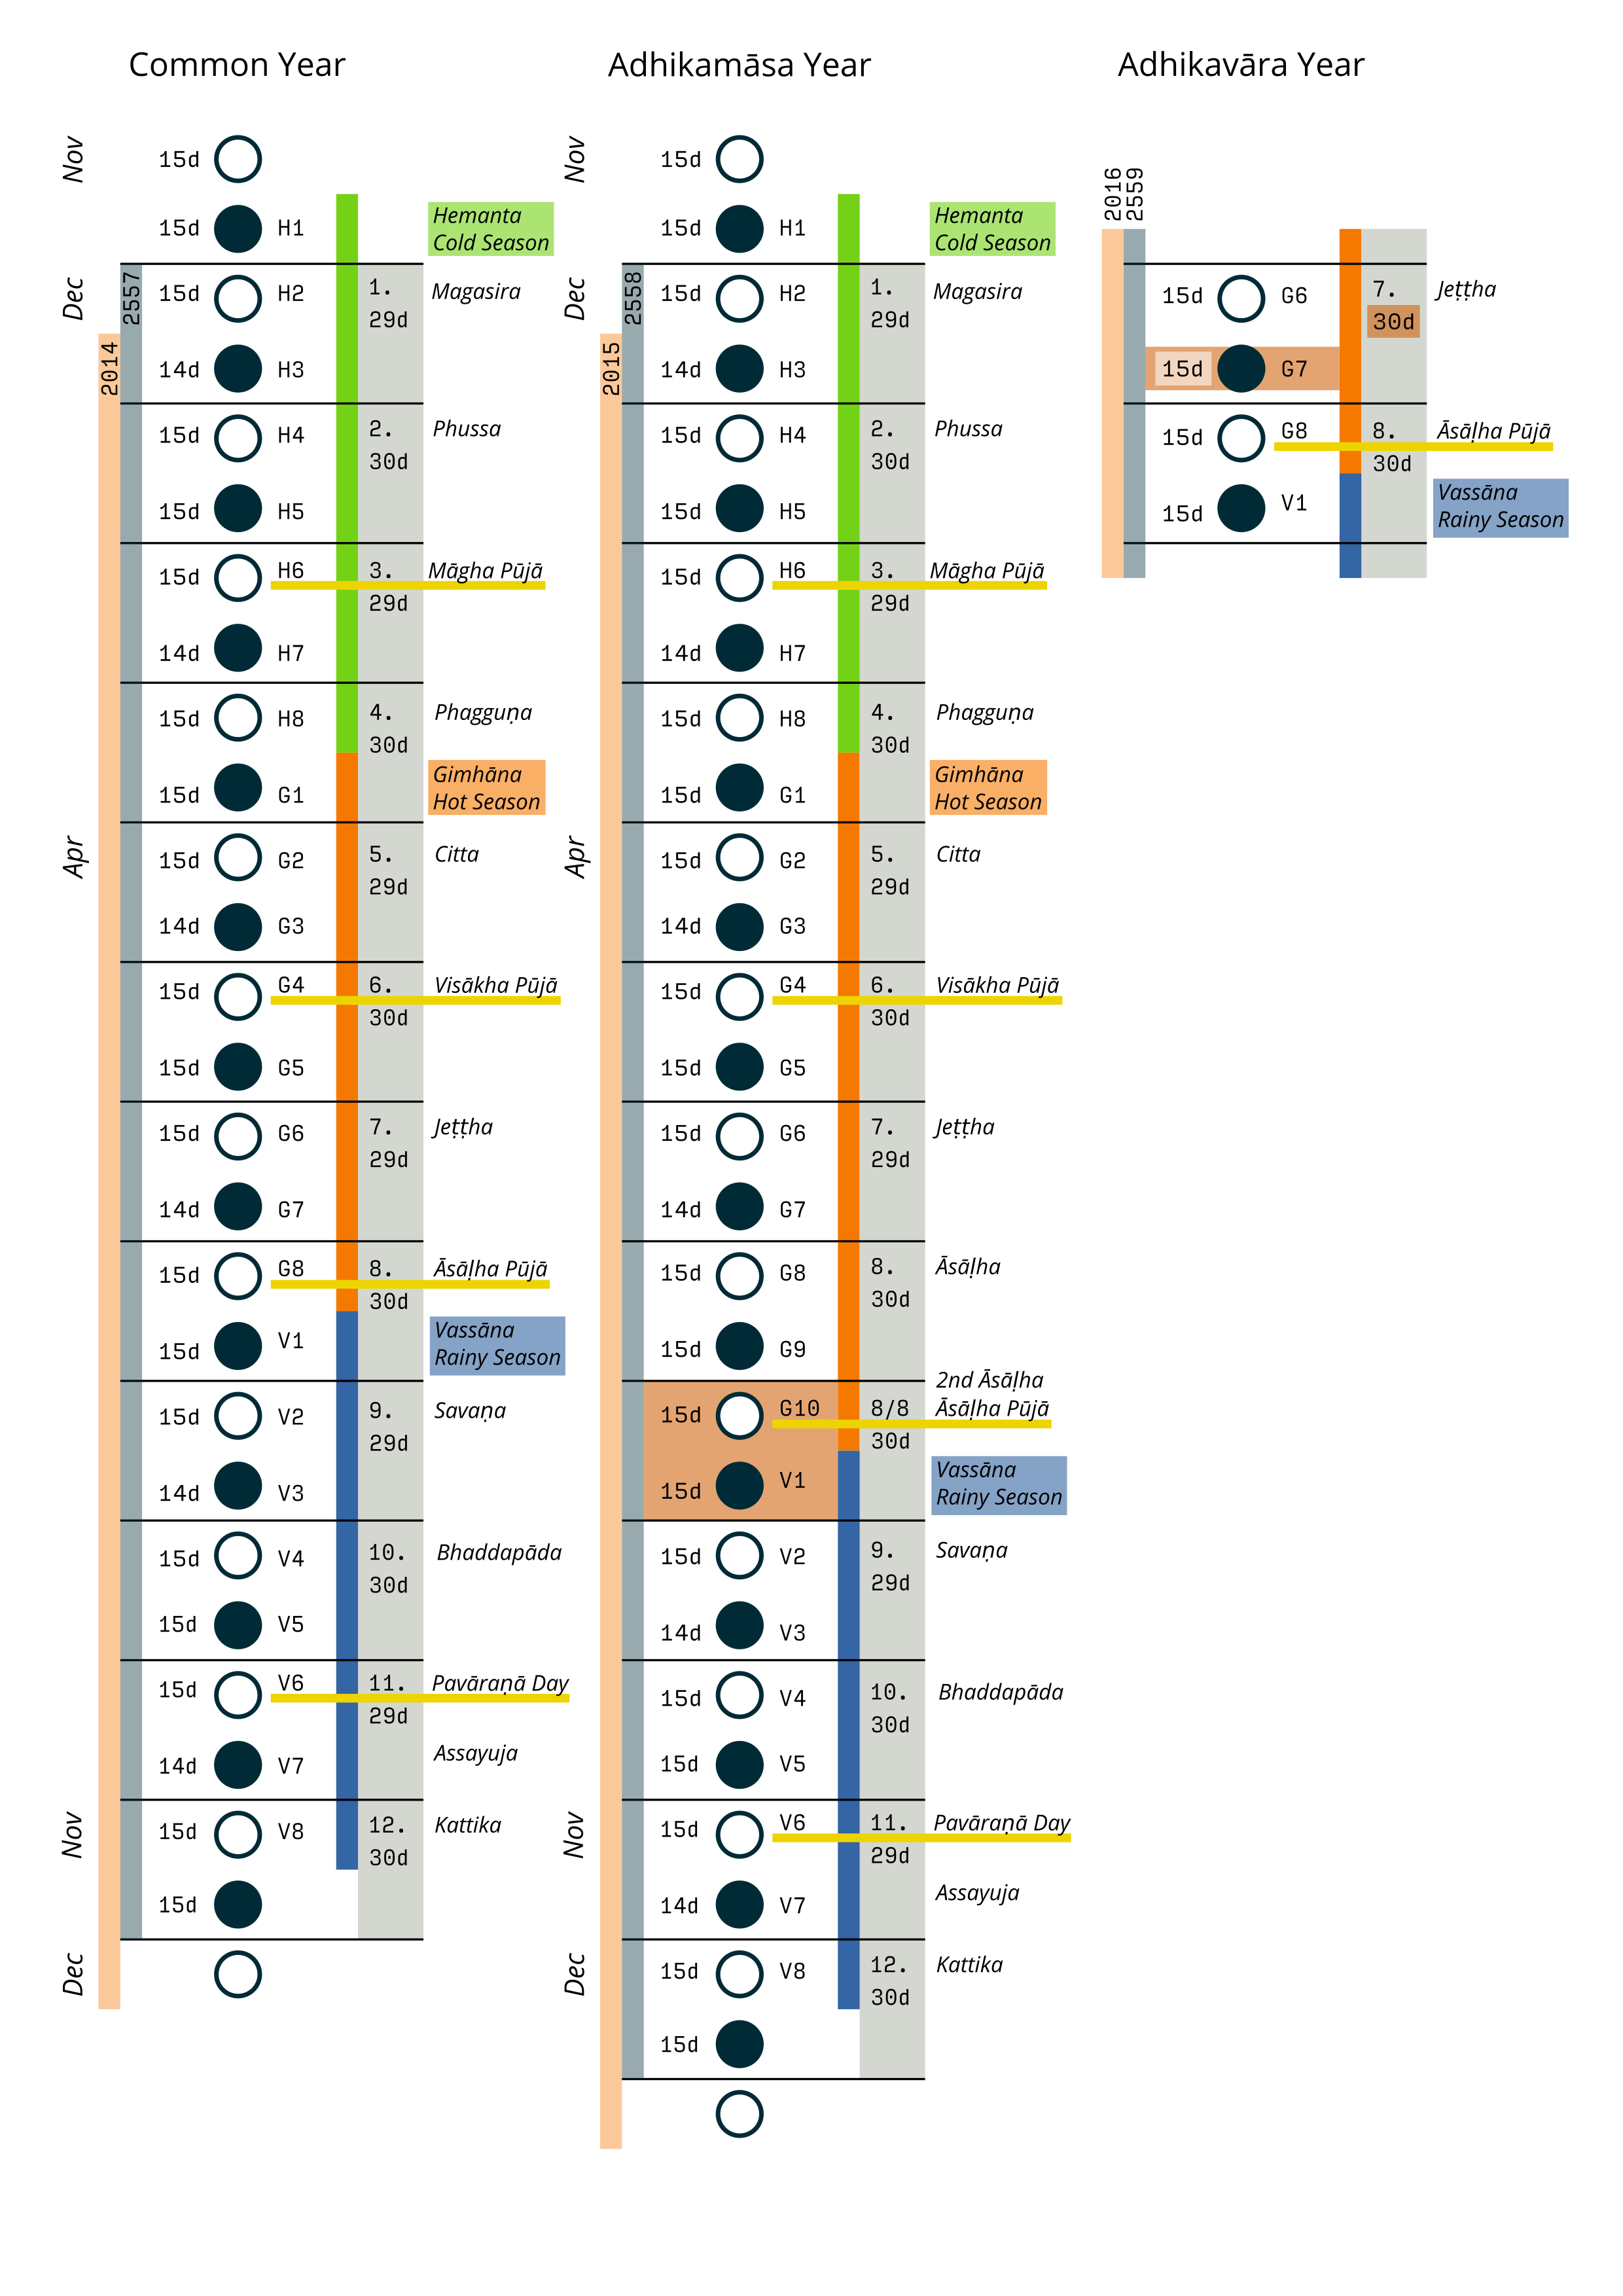
\includegraphics[width=\paperwidth]{common-adhikamasa-adhikavara.png}%
}

\fullpage{%
\label{year-2014}%
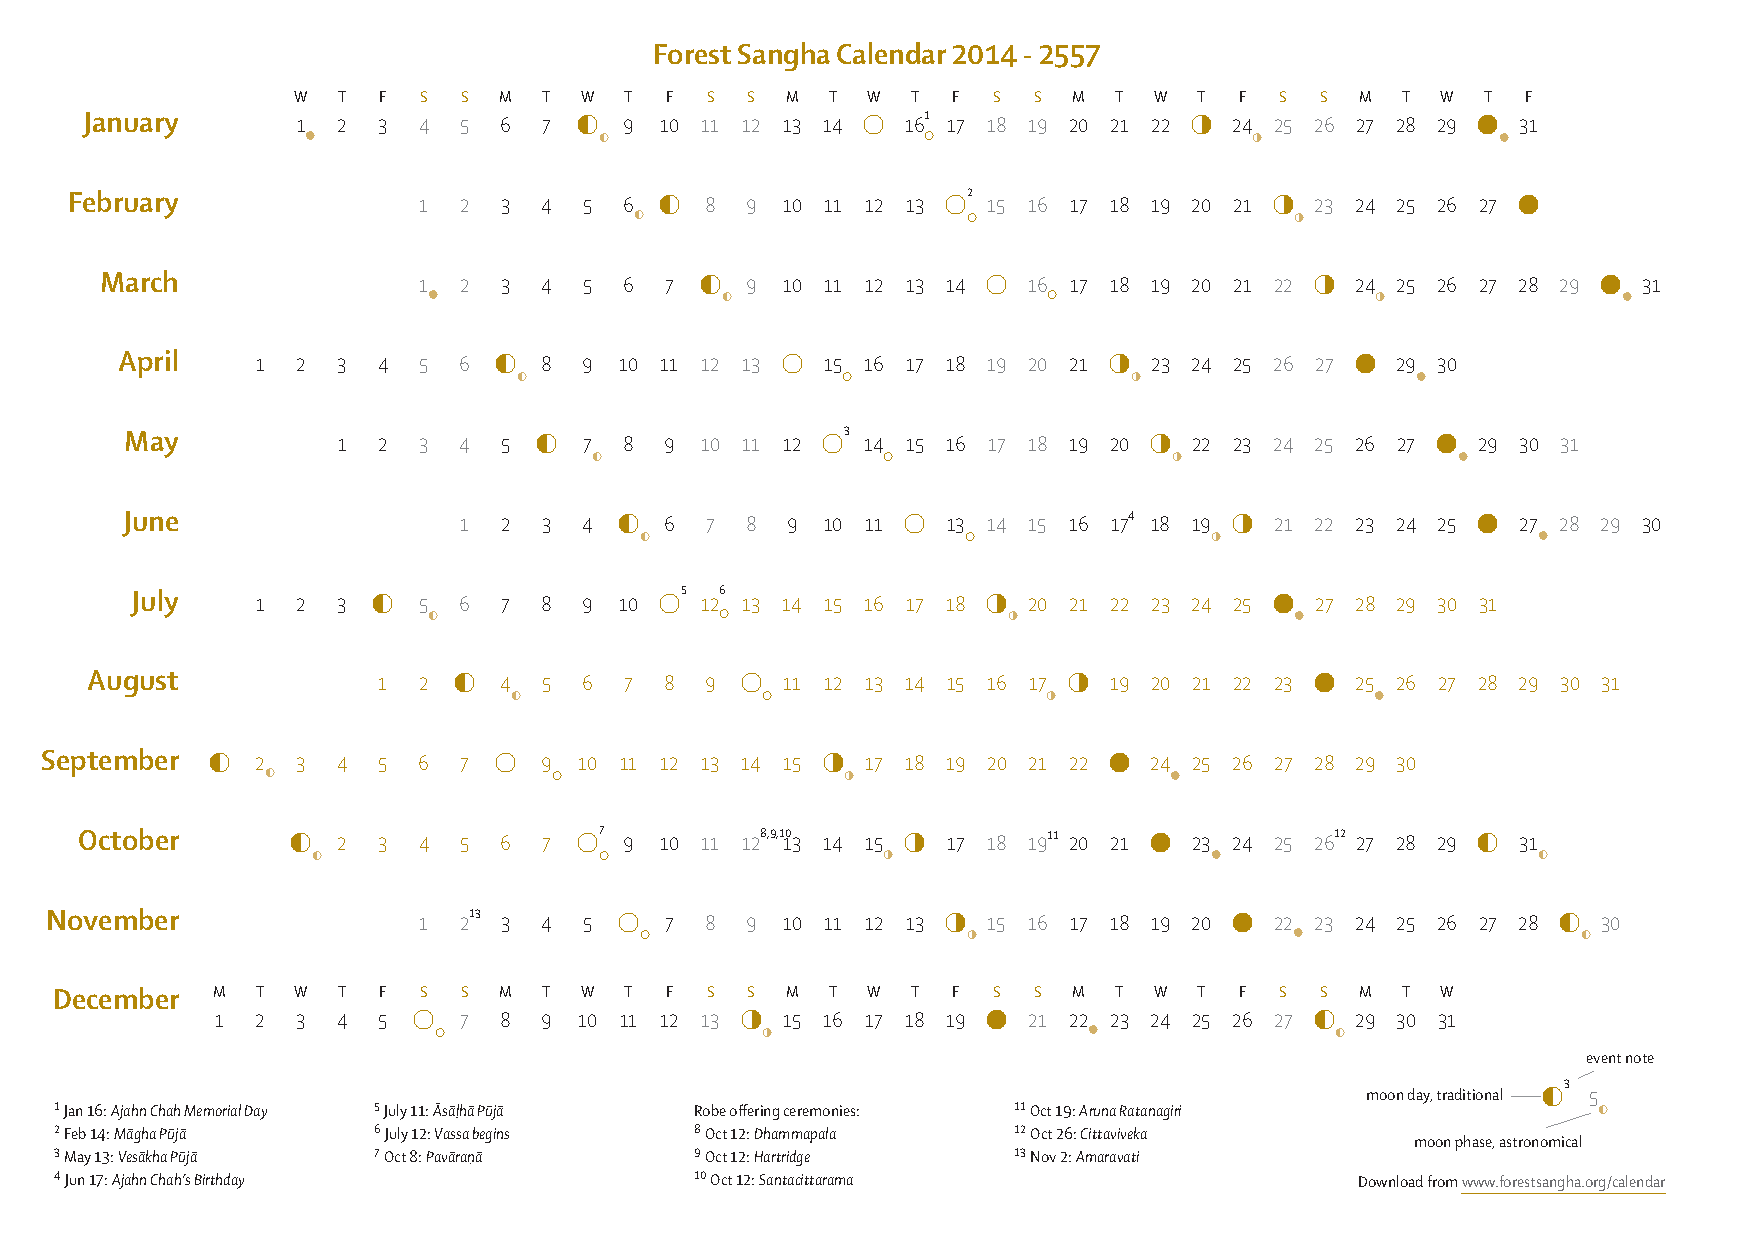
\includegraphics[angle=90,width=\paperwidth]{2014-fs-year-planner-A4.pdf}%
}

\fullpage{%
\label{year-2015}%
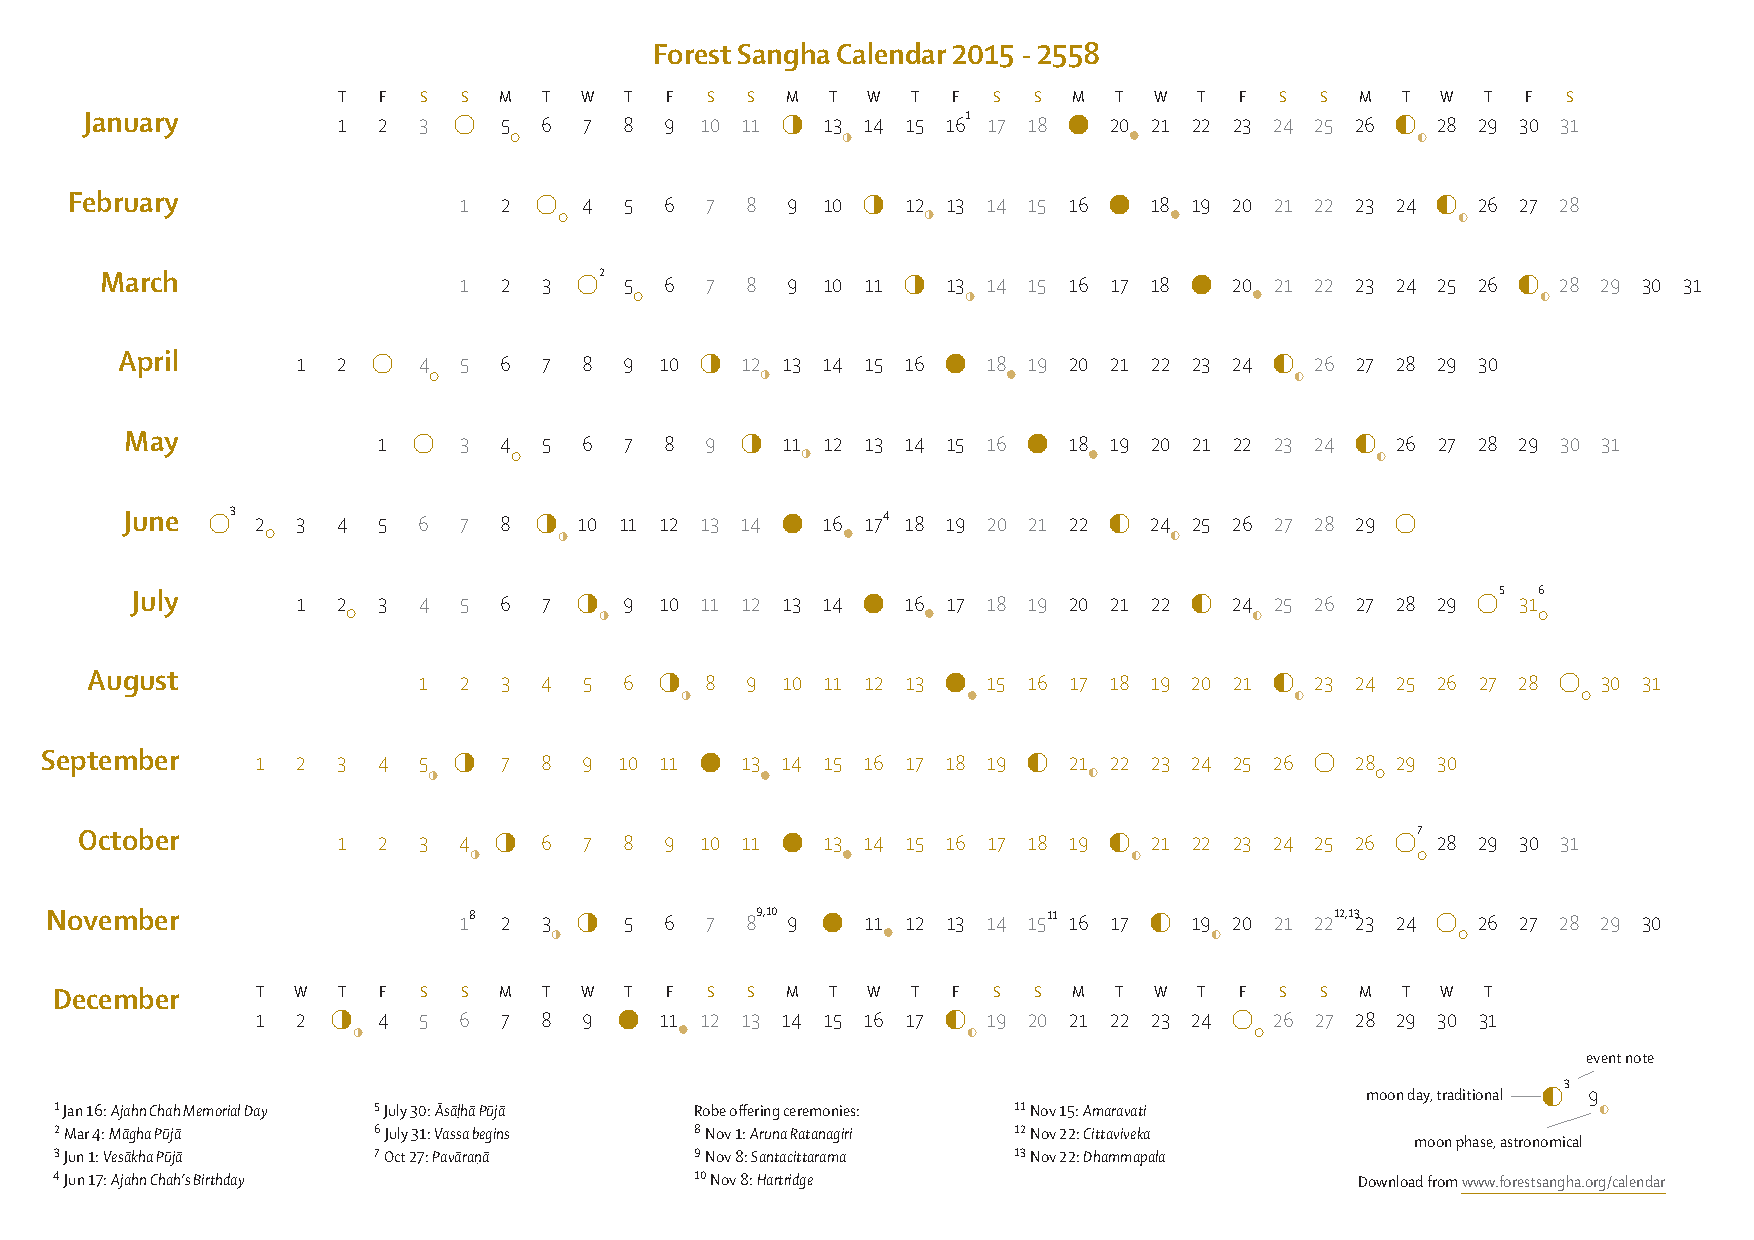
\includegraphics[angle=90,width=\paperwidth]{2015-fs-year-planner-A4.pdf}%
}

\fullpage{%
\label{year-2016}%
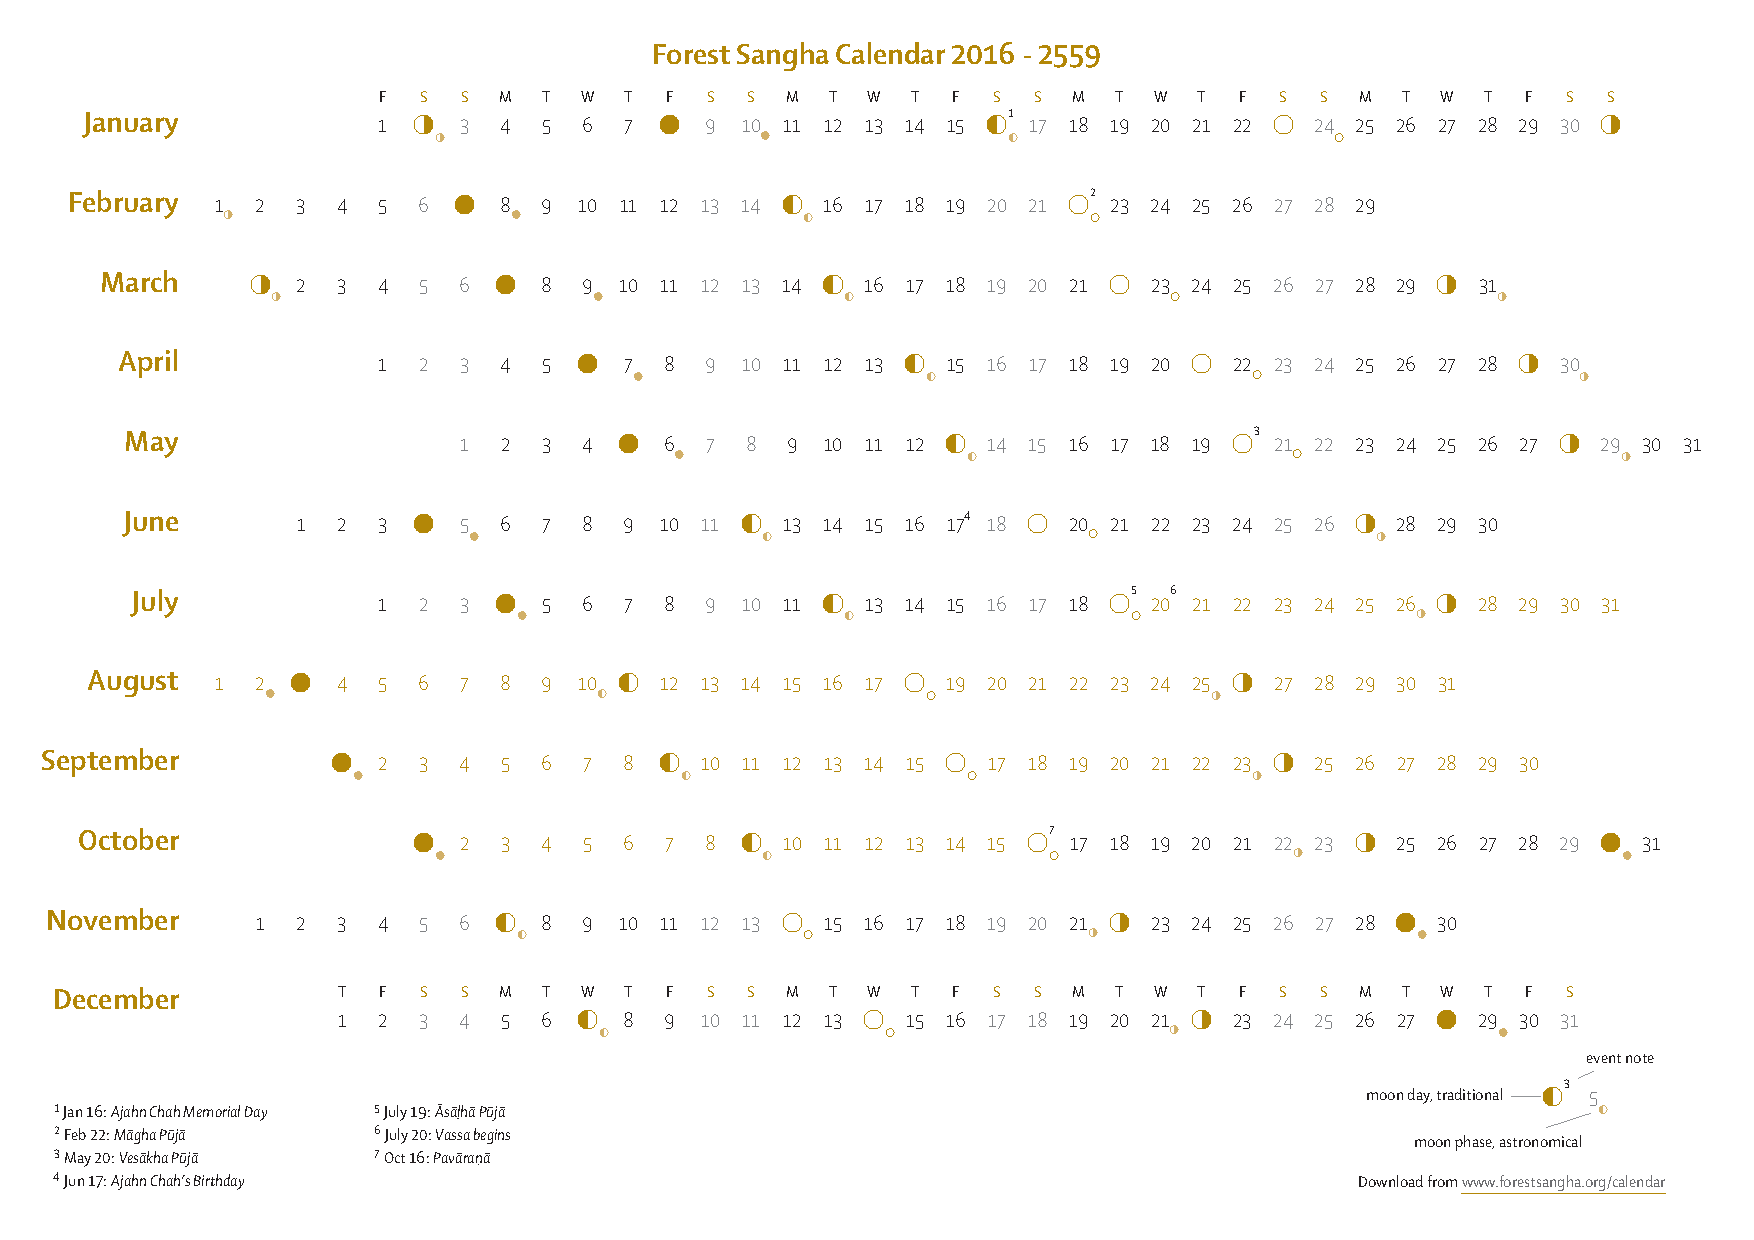
\includegraphics[angle=90,width=\paperwidth]{2016-fs-year-planner-A4.pdf}%
}
% Emacs 25.0.50.1 (Org mode 8.2.10)
\end{document}